% =====================================================================
% BAB IV IMPLEMENTASI DAN EVALUASI
% =====================================================================

\chapter{IMPLEMENTASI DAN EVALUASI}
\label{ch:evaluasi}

% Bab ini menjelaskan bagaimana rancangan pada BAB III diwujudkan menjadi sistem AXIS yang berjalan. Pembahasan dimulai dari implementasi arsitektur inti, dilanjutkan dengan hasil antarmuka web yang dialami pengguna, lalu ditutup dengan evaluasi. Urutan ini dipilih agar pembaca melihat hubungan langsung antara rancangan konseptual, realisasi teknis, dan bukti pengujiannya.

\section{Implementasi AXIS}
\label{sec:implementasi}

\subsection{Arsitektur Sistem}
\label{sec:implementasi-arsitektur-inti}

Rancangan AXIS direalisasikan sebagai arsitektur berlapis. Antarmuka web menjadi ruang interaksi pengguna. Layanan \textit{backend} menangani autentikasi, sesi, data pengguna, dan penghubung ke layanan agentik. Layanan agentik menjalankan alur keputusan percakapan, mulai dari pengayaan bahasa, pengambilan memori, kebijakan dialog, PHQ-9, hingga \textit{guardrail}. Penyimpanan data dibagi sesuai perannya: PostgreSQL untuk data relasional dan vektor, Neo4j untuk memori relasional, serta Redis untuk \textit{state} sementara dan pengendalian penggunaan. Komponen suara terhubung ke layanan STT/TTS dan audio respons dikembalikan ke klien sebagai \textit{payload} suara, bukan sebagai kontribusi penyimpanan utama. Arsitektur implementasi ditunjukkan pada Gambar \ref{fig:system-arch}.

\begin{figure}[!htbp]
  \centering
  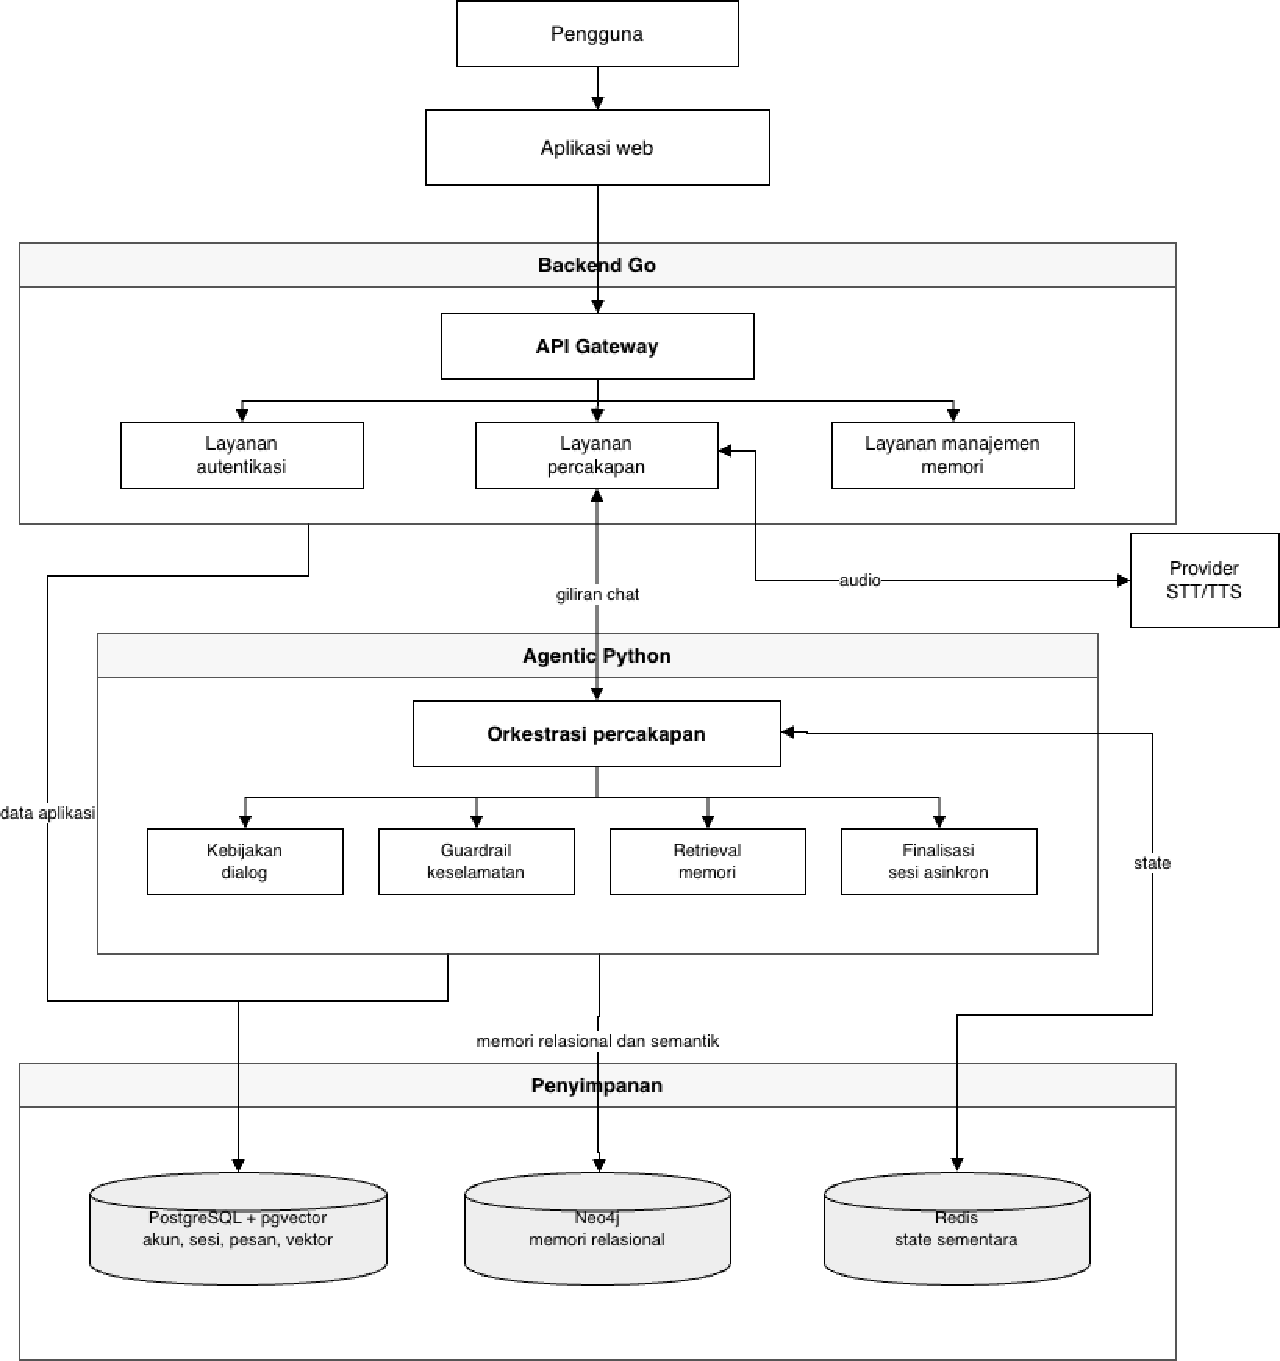
\includegraphics[width=0.95\textwidth]{figures/system_architecture.pdf}
  \caption[Arsitektur implementasi sistem AXIS]{Arsitektur implementasi AXIS yang memisahkan antarmuka web, layanan \textit{backend}, \textit{pipeline} agentik, dan penyimpanan memori.}
  \label{fig:system-arch}
\end{figure}

Redis digunakan sebagai lapisan pendukung, bukan kontribusi utama penelitian. Perannya adalah menyimpan state sementara, membantu pengendalian penggunaan, dan menyiapkan sistem untuk evaluasi pengguna nyata agar layanan tidak mudah disalahgunakan. Dengan cara ini, pembatasan teknis tetap hadir tanpa mengambil fokus dari kontribusi utama, yaitu percakapan, mood/PHQ-9, dan memori jangka panjang.

Karena kualitas respons dan ekstraksi memori sangat dipengaruhi oleh model bahasa yang dipakai, konfigurasi model perlu dinyatakan secara eksplisit tanpa mengunci laporan pada satu nama model tertentu. Implementasi AXIS menyediakan lapisan konfigurasi penyedia yang dapat diarahkan ke OpenAI, Gemini, atau model lokal berbasis MLX. Setiap komponen menggunakan profil model yang berbeda sesuai perannya: generasi respons, peringkasan sesi, ekstraksi graf, penilaian PHQ-9, dan penulisan ulang \textit{guardrail}. Tabel \ref{tab:llm-config} merangkum profil tersebut sebagaimana direalisasikan pada konfigurasi layanan agentik.

\begin{table}[!htbp]
\centering
\caption{Profil konfigurasi model bahasa pada layanan agentik AXIS}
\label{tab:llm-config}
{\footnotesize
\begin{tabularx}{\textwidth}{|>{\raggedright\arraybackslash}p{3cm}|>{\raggedright\arraybackslash}p{3.5cm}|>{\raggedright\arraybackslash}p{2.2cm}|>{\raggedright\arraybackslash}X|}
\hline
\rowcolor{tableheadgray}
\textbf{Komponen} & \textbf{Profil konfigurasi} & \textbf{Temperatur} & \textbf{Fungsi} \\
\hline
Response generator & Model generatif utama provider aktif & 1,0 & Menyusun respons utama dan mendukung streaming teks. \\
\hline
Session summarizer & Model kuat provider aktif & 1,0 & Merangkum sesi sebelum finalisasi memori. \\
\hline
KG extractor & Model ekstraksi terstruktur provider aktif & 1,0 & Mengekstrak kandidat node dan relasi memori dari pesan pengguna. \\
\hline
PHQ-9 \textit{judge/scorer} & Model deterministik/ringan penyedia aktif & 0,0 & Menginterpretasi jawaban pengguna terhadap item PHQ-9 secara terstruktur. \\
\hline
PHQ-9 feedback & Model generatif kuat provider aktif & 1,0 & Membentuk umpan balik akhir PHQ-9 dengan bahasa non-diagnostik. \\
\hline
\textit{Guardrail} rewrite & Model generatif kuat provider aktif & 1,0 & Menulis ulang respons yang melanggar batas keluaran. \\
\hline
\end{tabularx}
}
\end{table}

Pada implementasi, pemetaan profil tersebut dilakukan melalui konfigurasi penyedia LLM dan variabel model per penyedia. Dengan demikian, eksperimen dapat dijalankan menggunakan Gemini, OpenAI, atau model lokal tanpa mengubah topologi \textit{pipeline}. Laporan ini memakai istilah profil model agar hasil dapat direplikasi berdasarkan konfigurasi aktual yang dipasang pada saat pengujian, bukan berdasarkan nama model yang dapat berubah antar penyedia.

\subsection{Percakapan, CBT, dan \textit{Guardrail}}
\label{subsec:impl-pipeline-agentik}

Setiap pesan pengguna diproses melalui \textit{pipeline} agentik yang eksplisit. Topologi \textit{pipeline} ditunjukkan pada Gambar \ref{fig:langgraph-flow}, sedangkan aliran satu giliran percakapan ditunjukkan pada Gambar \ref{fig:seq-chat-turn}. Pembagian node membuat keputusan sistem dapat dilacak: pesan diperkaya secara linguistik, diperiksa dari sisi keselamatan, dipadukan dengan konteks memori, lalu diarahkan ke pola respons yang sesuai.

\begin{figure}[!htbp]
  \centering
  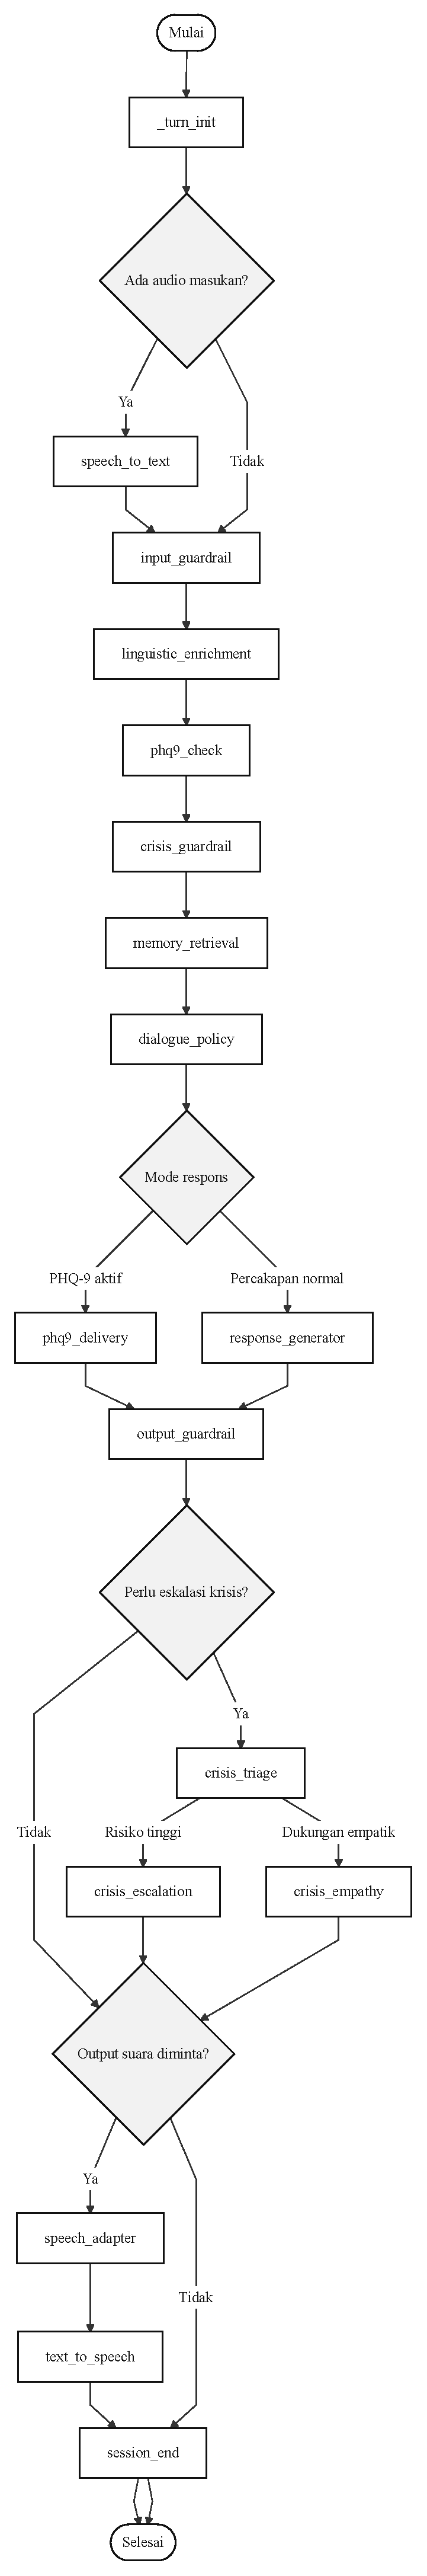
\includegraphics[width=0.95\textwidth,height=0.85\textheight,keepaspectratio]{figures/langgraph_flow.pdf}
  \caption[Topologi implementasi \textit{pipeline} agentik]{Topologi implementasi \textit{pipeline} agentik AXIS untuk memproses satu giliran percakapan secara bertahap.}
  \label{fig:langgraph-flow}
\end{figure}

\begin{figure}[!htbp]
  \centering
  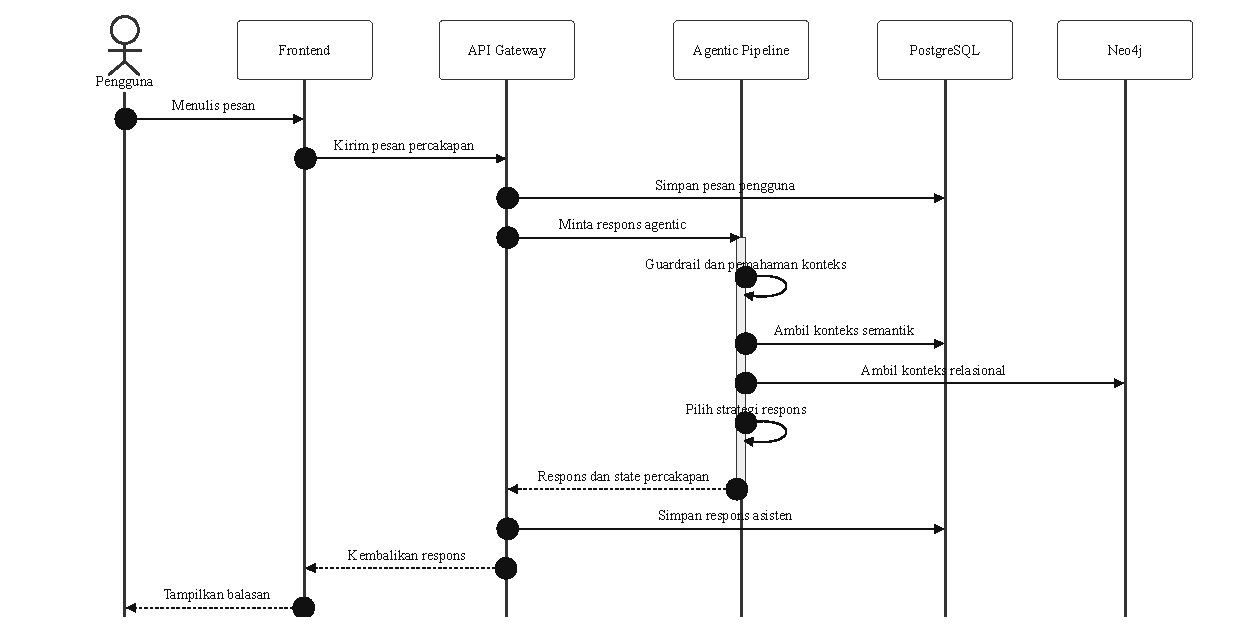
\includegraphics[width=0.95\textwidth]{figures/seq_chat_turn.pdf}
  \caption[Aliran pesan satu giliran teks]{Aliran pesan satu giliran teks dari antarmuka pengguna, layanan chat, \textit{pipeline} agentik, hingga respons kembali ke klien.}
  \label{fig:seq-chat-turn}
\end{figure}

Pengayaan linguistik digunakan agar AXIS dapat membaca bahasa pengguna dengan lebih sesuai konteks mahasiswa Indonesia. Bahasa Indonesia informal, istilah Inggris kampus, dan ekspresi campuran diperlakukan sebagai sinyal percakapan, bukan sebagai kesalahan bahasa. Hasil pengayaan ini memengaruhi bahasa respons dan membantu \textit{guardrail} memahami ungkapan tidak langsung.

Kebijakan dialog menjadi penghubung antara sinyal percakapan dan respons akhir. Implementasi alur CBT ditunjukkan pada Gambar \ref{fig:cbt-dialogue-flow-impl}. Jika PHQ-9 sedang aktif atau percakapan sedang berada pada jalur krisis, pemilihan teknik CBT dinonaktifkan agar sistem tidak mencampur skrining atau eskalasi dengan latihan reflektif. Jika pengguna menolak teknik yang baru ditawarkan, sistem menurunkan respons ke validasi agar percakapan tetap terasa sukarela. Jika sinyal percakapan cukup jelas, sistem memilih teknik seperti reframing, self-compassion, behavior activation, psychoeducation, atau thought record. Prinsipnya tetap sama seperti rancangan BAB III: teknik reflektif ditawarkan sebagai bantuan, bukan instruksi klinis.

\begin{figure}[!htbp]
  \centering
  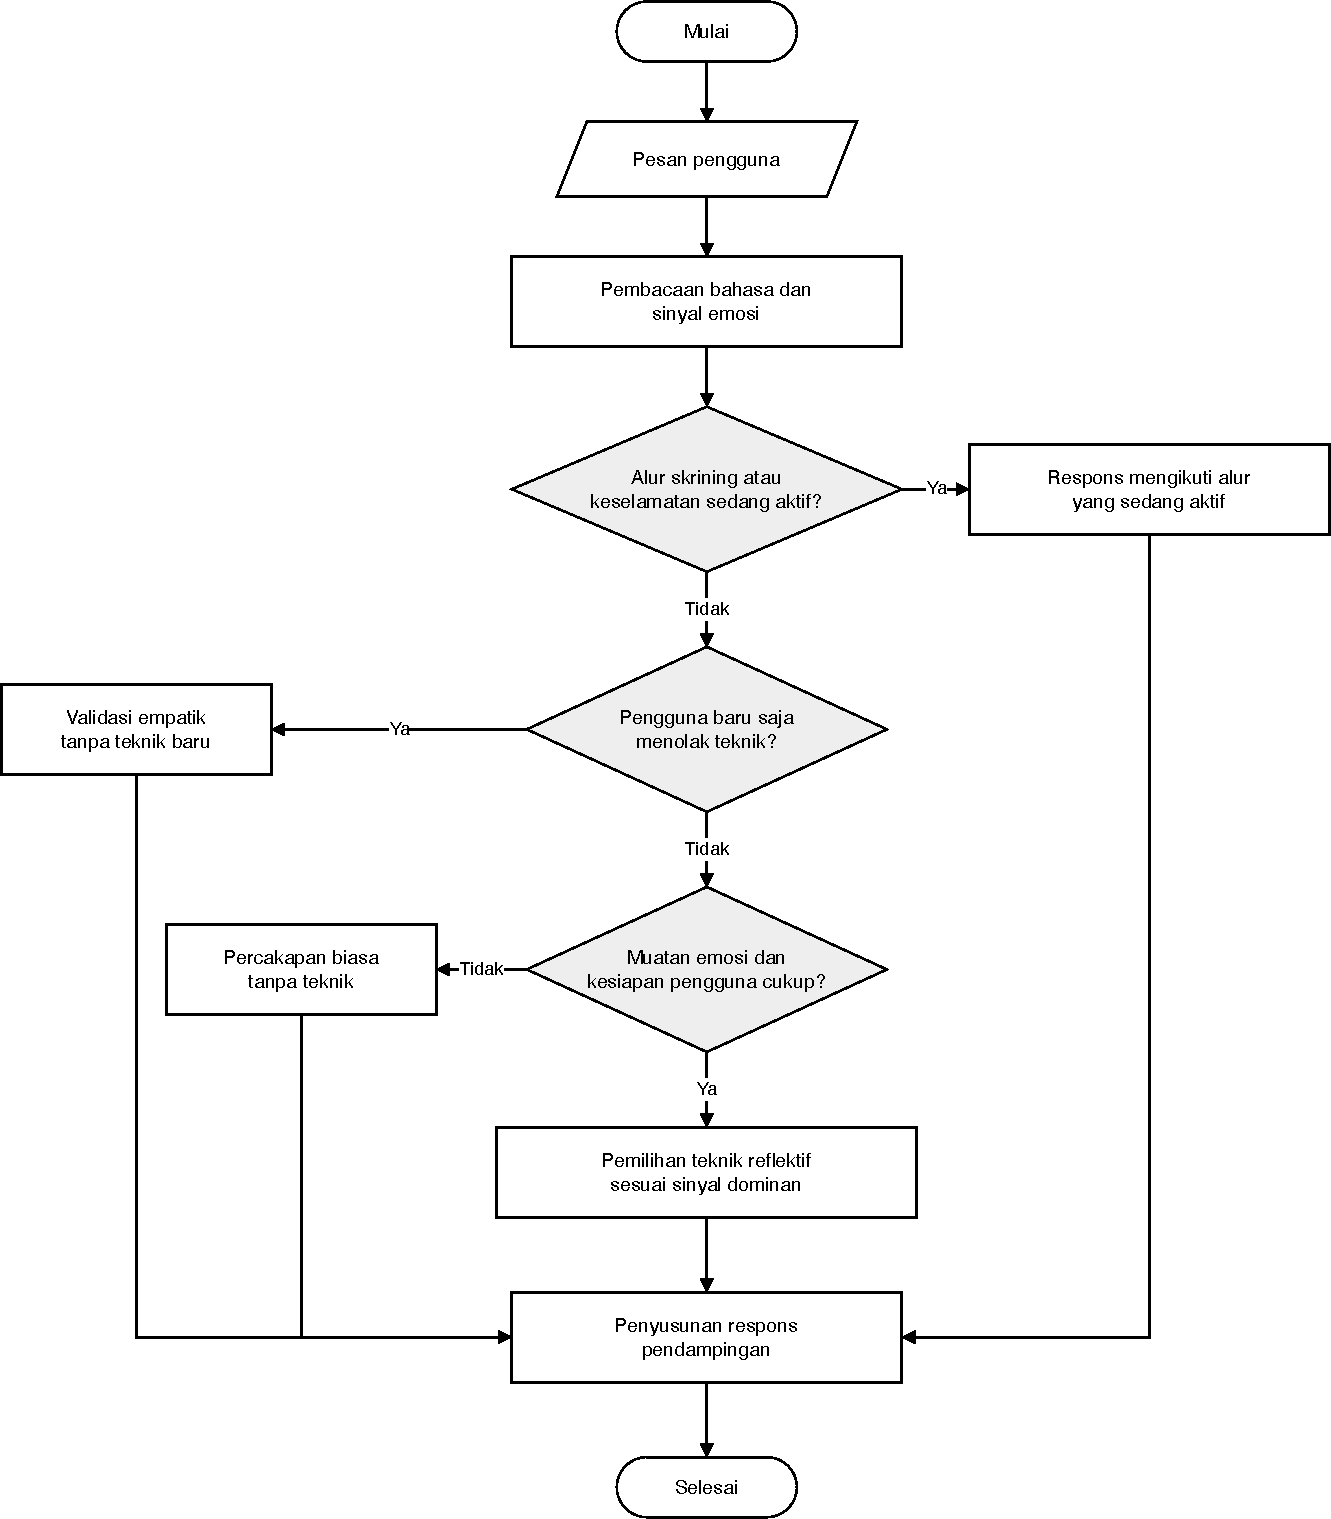
\includegraphics[width=0.9\textwidth]{figures/cbt_dialogue_flow.pdf}
  \caption[Implementasi alur pemilihan CBT]{Implementasi alur pemilihan teknik CBT berdasarkan sinyal percakapan, status PHQ-9, status krisis, dan penolakan pengguna.}
  \label{fig:cbt-dialogue-flow-impl}
\end{figure}

Pemilihan teknik CBT menggabungkan dua jalur: pencocokan sinyal deterministik dan penilai berbasis LLM untuk kasus yang lebih samar. Kebijakan dialog tidak langsung menawarkan teknik reflektif berat pada awal percakapan. Sistem mewajibkan giliran minimum sebelum teknik hasil keputusan otomatis, khususnya \textit{grounding}, dapat ditawarkan. Ambang keyakinan penilai dibuat lebih ketat untuk \textit{grounding} karena bobot intervensinya lebih besar dibanding validasi atau reframing. Pencocokan sinyal distorsi kognitif juga disyaratkan tetap disertai muatan emosi pada giliran yang sama, kecuali ketika pengguna sedang berada pada giliran lanjutan dari teknik reflektif yang sudah berjalan.

Kebijakan dialog juga menangani penolakan dan perpindahan status percakapan. Penolakan berturut-turut terhadap teknik yang berbeda menekan penawaran teknik baru untuk sementara. Status latihan reflektif yang sedang berjalan direset ketika percakapan ditandai sebagai krisis, sehingga latihan tersebut tidak berlanjut diam-diam setelah momen krisis berlalu. Perilaku ini diverifikasi melalui pengujian unit (Subbab~\ref{sec:evaluasi-fungsional}) dan studi kasus ilustratif pada Subbab~\ref{sec:evaluasi-komparatif}.

Rancangan reflektif memprioritaskan regulasi afek di atas penantangan pola pikir (Subbab~\ref{sec:rancangan-companionship}), sehingga distorsi kognitif yang muncul bersamaan afek akut (mis. pikiran katastrofik yang diutarakan bersamaan kepanikan) memerlukan mekanisme susulan agar tetap ditantang balik setelah giliran \textit{grounding} selesai, bukan dibiarkan lewat begitu saja. Ketika giliran sebelumnya adalah \textit{grounding} dan sebuah distorsi tercatat pada saat itu, sistem otomatis menawarkan \textit{reframing} atas distorsi tersebut pada giliran berikutnya, selama pengguna belum berpindah topik atau kehilangan muatan emosional. \textit{Prompt} penilai LLM mencatat nama distorsi pada bidang keluarannya bahkan ketika teknik yang dipilih adalah \textit{grounding}, sehingga mekanisme susulan ini punya informasi yang dibutuhkan untuk bekerja.

Mekanisme susulan ini diverifikasi dengan pemanggilan LLM nyata, dilaporkan pada Subbab~\ref{sec:evaluasi-fungsional}.

Frekuensi penyebutan nama pengguna dibatasi lewat pemeriksaan berbasis kode: sebelum setiap giliran, sistem memeriksa langsung riwayat giliran asisten sebelumnya untuk mendeteksi apakah nama pengguna baru saja dipakai, lalu menyisipkan instruksi kontekstual yang sesuai (larangan mutlak jika dipakai pada giliran tepat sebelumnya, larangan lunak jika dipakai pada dua giliran terakhir). Mekanisme serupa juga diterapkan pada pola menutup giliran dengan pertanyaan: jika beberapa giliran asisten berturut-turut sama-sama berakhir dengan tanda tanya, sistem menyisipkan instruksi agar giliran berikutnya ditutup sebagai pernyataan reflektif atau observasi, bukan pertanyaan lagi, sehingga ritme percakapan tidak seragam sepanjang sesi. Pola gaung-parafrasa di awal giliran diperlakukan berbeda karena mendeteksinya secara mekanis dari kode jauh lebih sulit dibanding mendeteksi kemunculan sebuah nama atau tanda baca penutup. Efektivitas ketiga mekanisme ini diukur pada Subbab~\ref{sec:evaluasi-fungsional}.

\textit{Guardrail} diimplementasikan pada beberapa titik \textit{pipeline} sebagai pagar bagi kebijakan dialog di atas, bukan sebagai pengganti percakapan empatik. Pemeriksaan awal menangkap sinyal eksplisit pada pesan pengguna. Pemeriksaan lanjutan membaca sinyal yang lebih samar. Pemeriksaan keluaran memastikan respons tidak membuat klaim klinis, tidak memberi instruksi berbahaya, dan tetap berada pada batas peran pendamping. Pada risiko tinggi, sistem mengalihkan respons ke rujukan bantuan. Alur eskalasi krisis ditunjukkan pada Gambar \ref{fig:crisis-flow}.

\begin{figure}[!htbp]
  \centering
  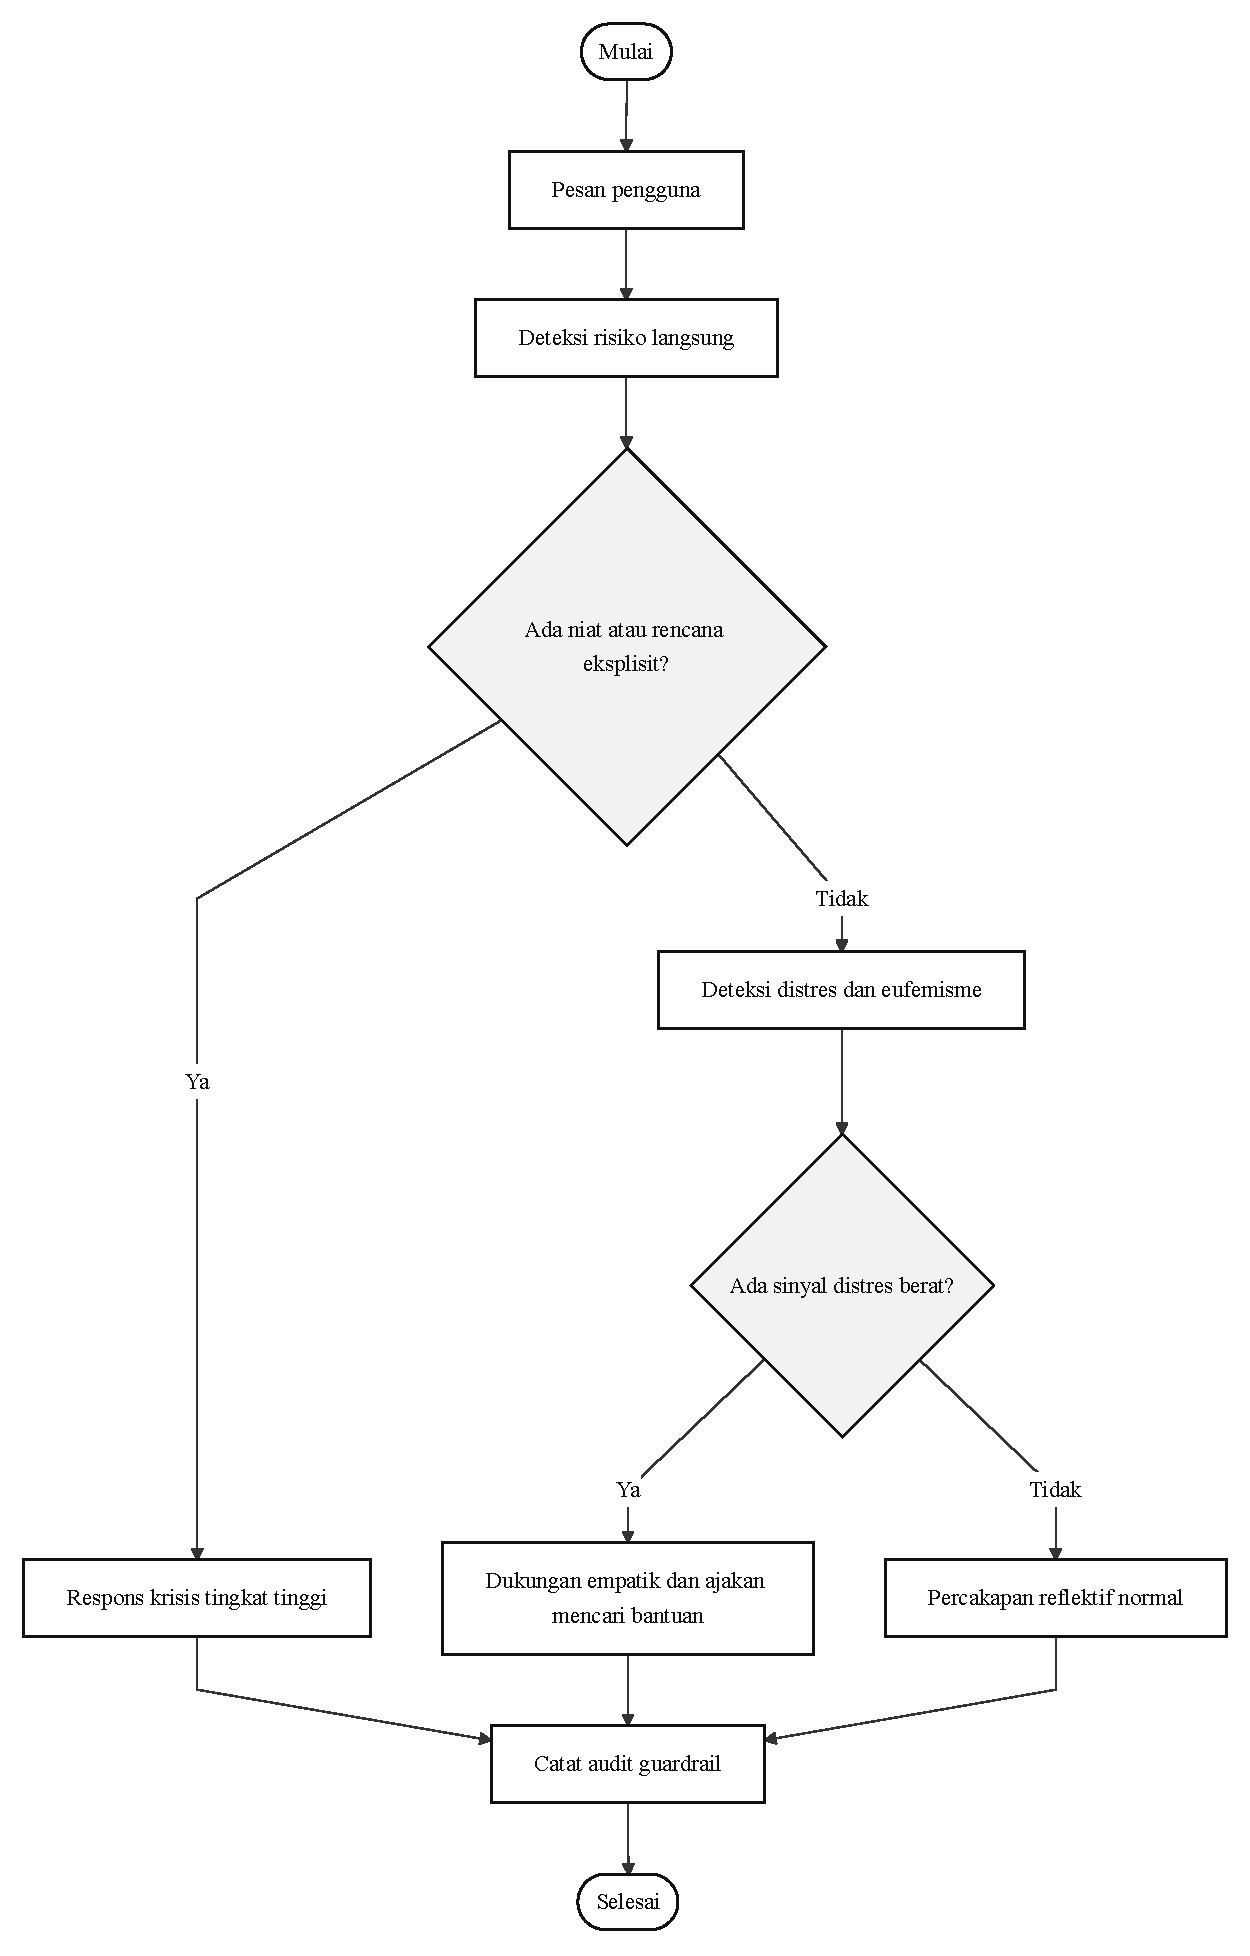
\includegraphics[width=0.85\textwidth]{figures/crisis_tier_flow.pdf}
  \caption[Implementasi alur respons krisis]{Implementasi alur respons krisis yang membedakan percakapan normal, distres umum, dan risiko tinggi.}
  \label{fig:crisis-flow}
\end{figure}

\textit{Guardrail} tidak diposisikan sebagai fitur utama yang ingin ditonjolkan, tetapi sebagai syarat agar percakapan pendamping tetap bertanggung jawab.
\label{subsec:impl-guardrail-phq9}

\subsection{Mood Harian dan PHQ-9}
\label{subsec:impl-mood-phq9}

Mood harian diimplementasikan sebagai catatan satu nilai suasana hati per pengguna per tanggal. Nilai ini berada pada rentang sangat sedih hingga sangat senang. \textit{Backend} menyimpan nilai tersebut, lalu layanan agentik mengambil mood hari ini dan tren singkat beberapa hari terakhir sebagai konteks percakapan. Sinyal ini tidak dipakai untuk mendiagnosis pengguna, melainkan membantu AXIS menyesuaikan nada respons.

PHQ-9 diimplementasikan sebagai \textit{state machine} percakapan. Sistem menyimpan fase skrining, item aktif, jawaban pengguna, dan status penawaran. Dengan state tersebut, PHQ-9 dapat berjalan bertahap di dalam chat, bukan sebagai formulir terpisah. Alur implementasinya ditunjukkan pada Gambar \ref{fig:phq9-state-machine-impl}.

\begin{landscape}
\begin{center}
  \centering
  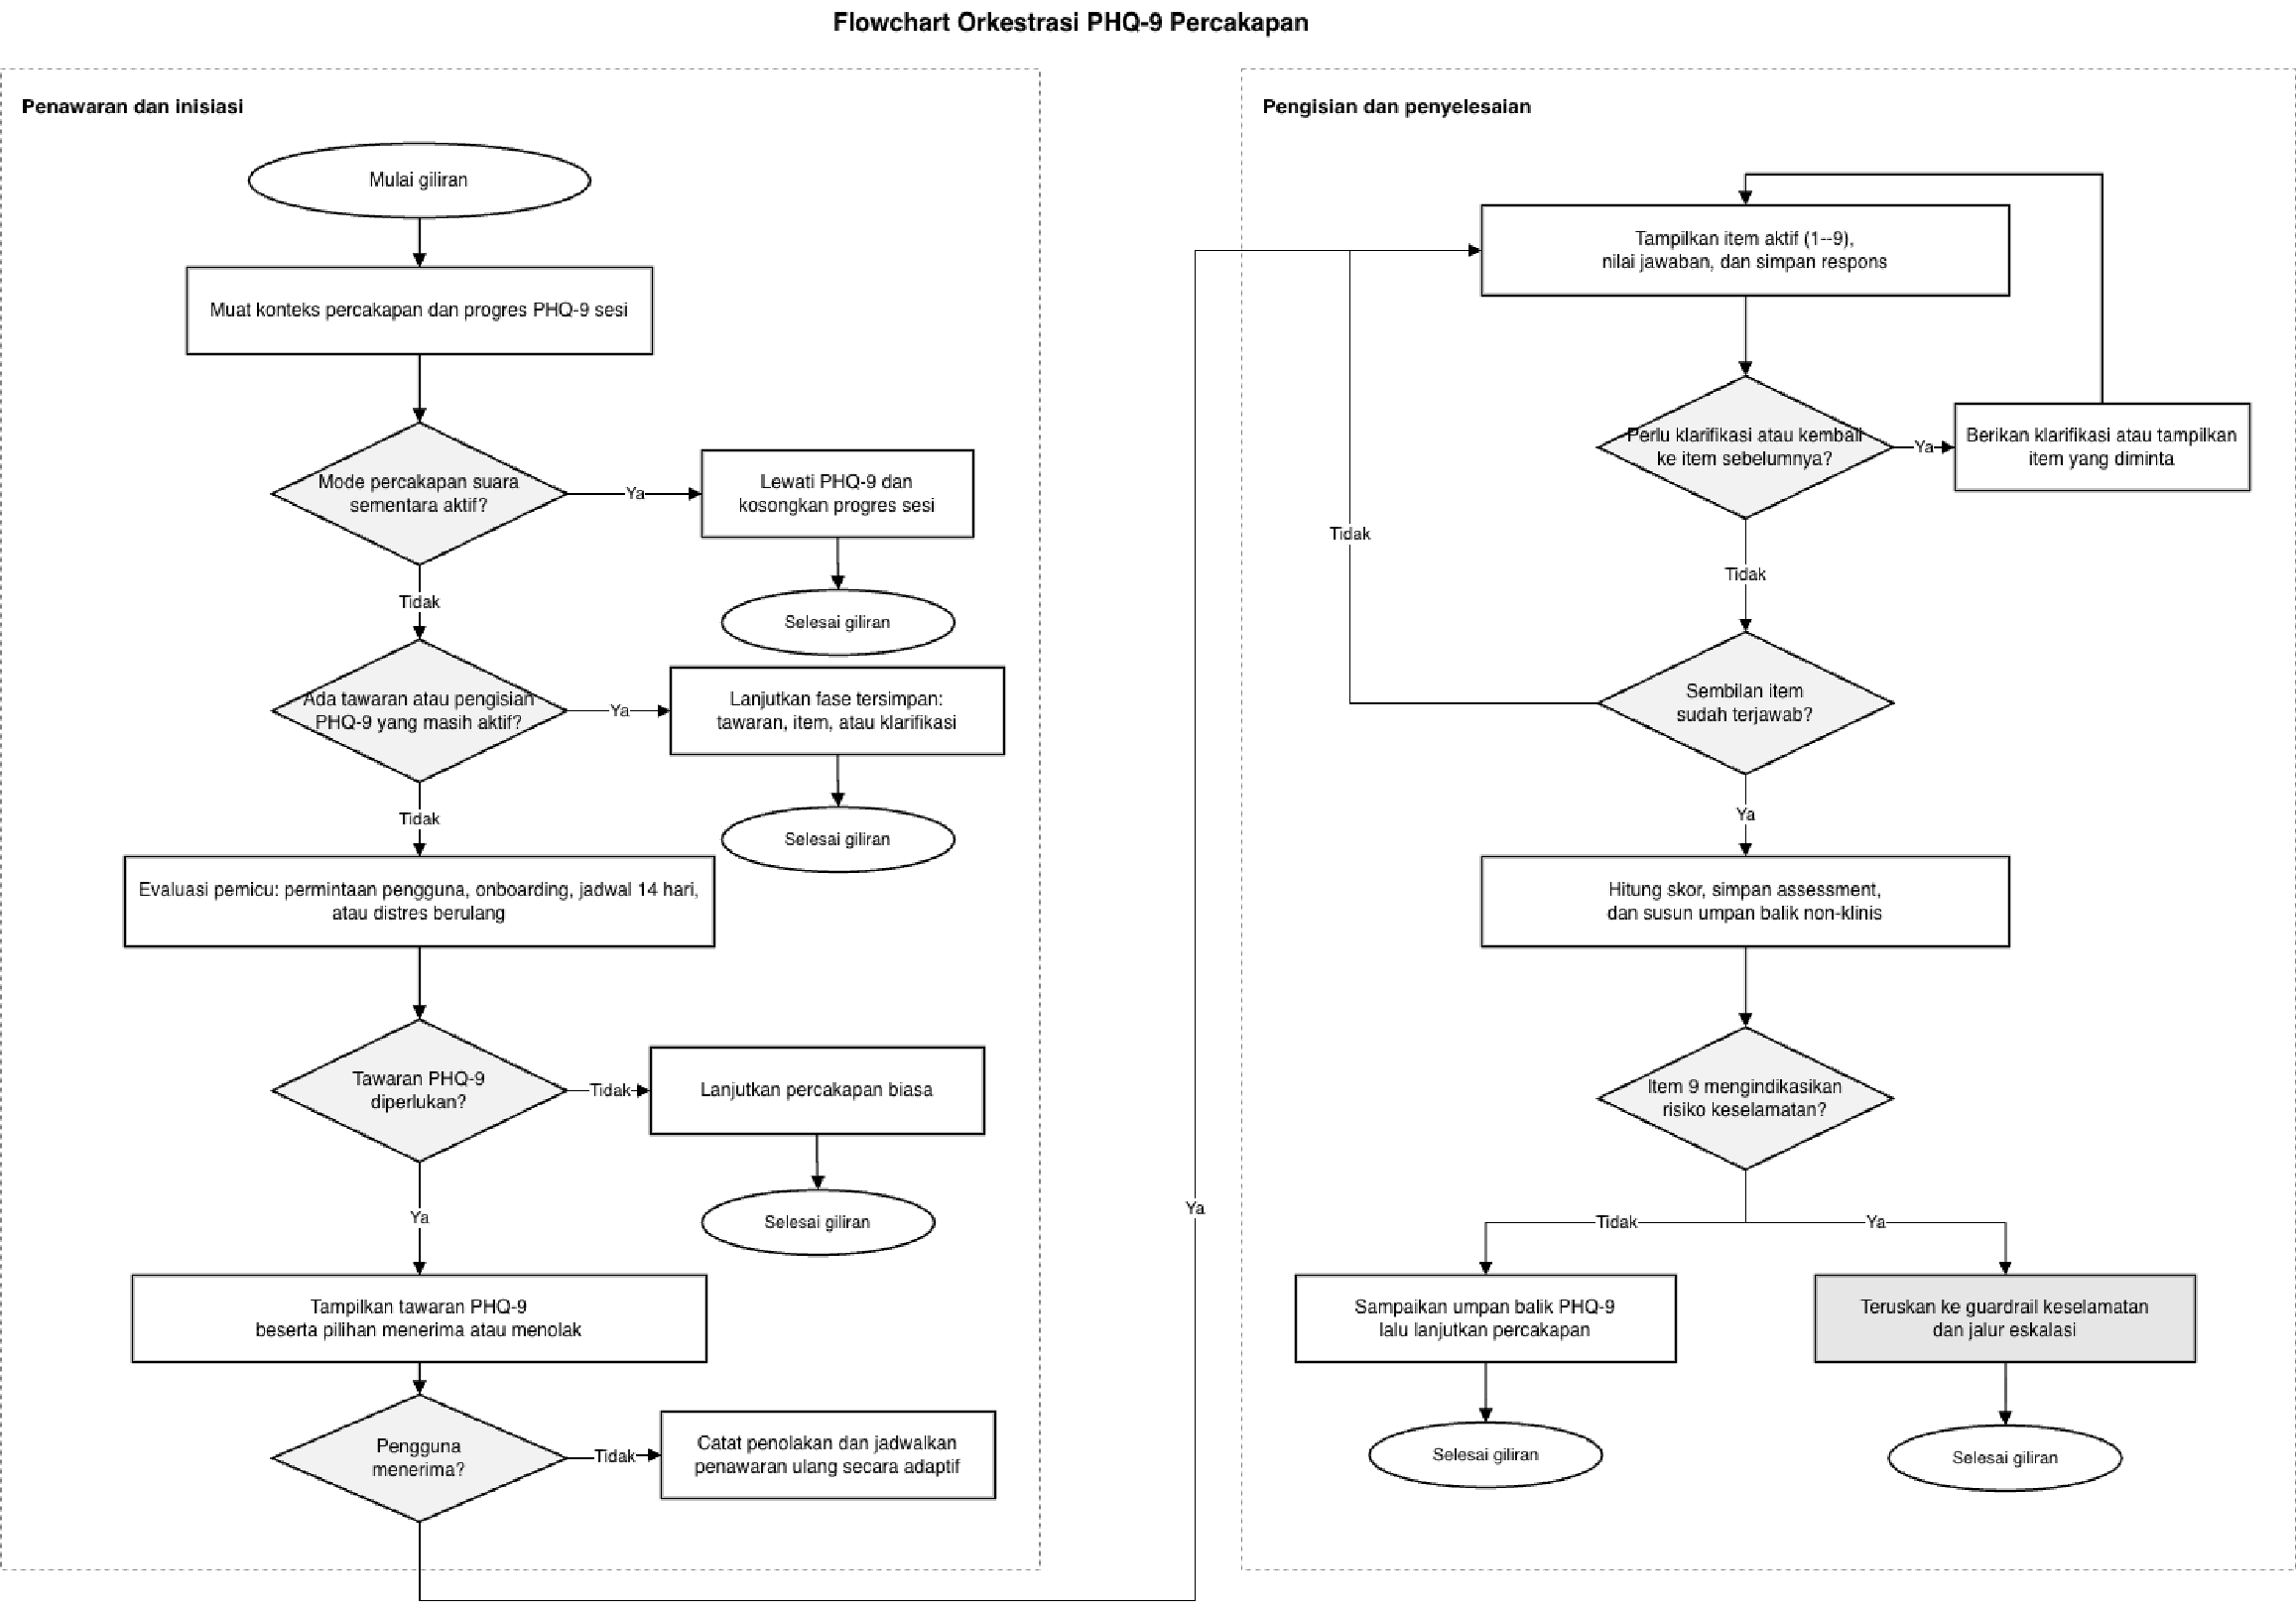
\includegraphics[width=0.98\linewidth,height=0.92\textheight,keepaspectratio]{figures/phq9_state_machine.pdf}
  \captionof{figure}[Flowchart implementasi PHQ-9]{Flowchart implementasi PHQ-9 percakapan dari penawaran, pengisian item, penyelesaian, hingga eskalasi keselamatan.}
  \label{fig:phq9-state-machine-impl}
\end{center}
\end{landscape}

Ketika hasil PHQ-9 selesai dihitung, sistem menyimpan hasilnya sebagai \textit{assessment}, bukan sebagai pengalaman hidup biasa. Pemisahan ini penting karena jawaban terhadap item kuesioner tidak selalu layak menjadi memori jangka panjang. Yang dapat menjadi memori adalah refleksi personal pengguna setelah asesmen, bukan administrasi item PHQ-9 itu sendiri.

\subsection{Memori Jangka Panjang}
\label{subsec:impl-memori-jangka-panjang}

Memori jangka panjang diimplementasikan sebagai arsitektur hibrid berbasis \textit{knowledge graph}. Neo4j menjadi sumber utama untuk node, relasi, dan status \textit{lifecycle} memori, sedangkan pgvector berperan sebagai cermin semantik untuk pencarian berbasis kemiripan. Dengan \textit{framing} ini, klaim utama AXIS bukan bahwa sistem memakai \textit{knowledge graph} secara murni tanpa vektor, melainkan bahwa relasi graf menjadi struktur pemahaman utama, sementara vektor membantu menemukan kandidat memori yang relevan secara semantik. Skema graf yang digunakan ditunjukkan pada Gambar \ref{fig:kg-schema}. Node dan relasi utama diringkas pada Tabel \ref{tab:node-relasi-utama}. Ekstraksi node Topic tidak dibatasi pada kosakata tetap, tetapi \textit{prompt} ekstraksinya (Lampiran~\ref{lamp:agentic-prompts-kg}) diberi contoh label bertema kehidupan mahasiswa yang selaras dengan enam area kalibrasi domain pada Subbab~\ref{sec:batasan-masalah}: tekanan akademik, relasi kampus (termasuk peran khusus \textit{dosen pembimbing} pada node Subject), keluarga, organisasi, identitas diri, dan transisi karier. Pendekatan ini bersifat contoh yang mengarahkan, bukan enumerasi tertutup, sehingga topik pengguna non-mahasiswa tetap dapat diekstrak secara bebas ketika tidak relevan dengan area tersebut.

\begin{figure}[!htbp]
  \centering
  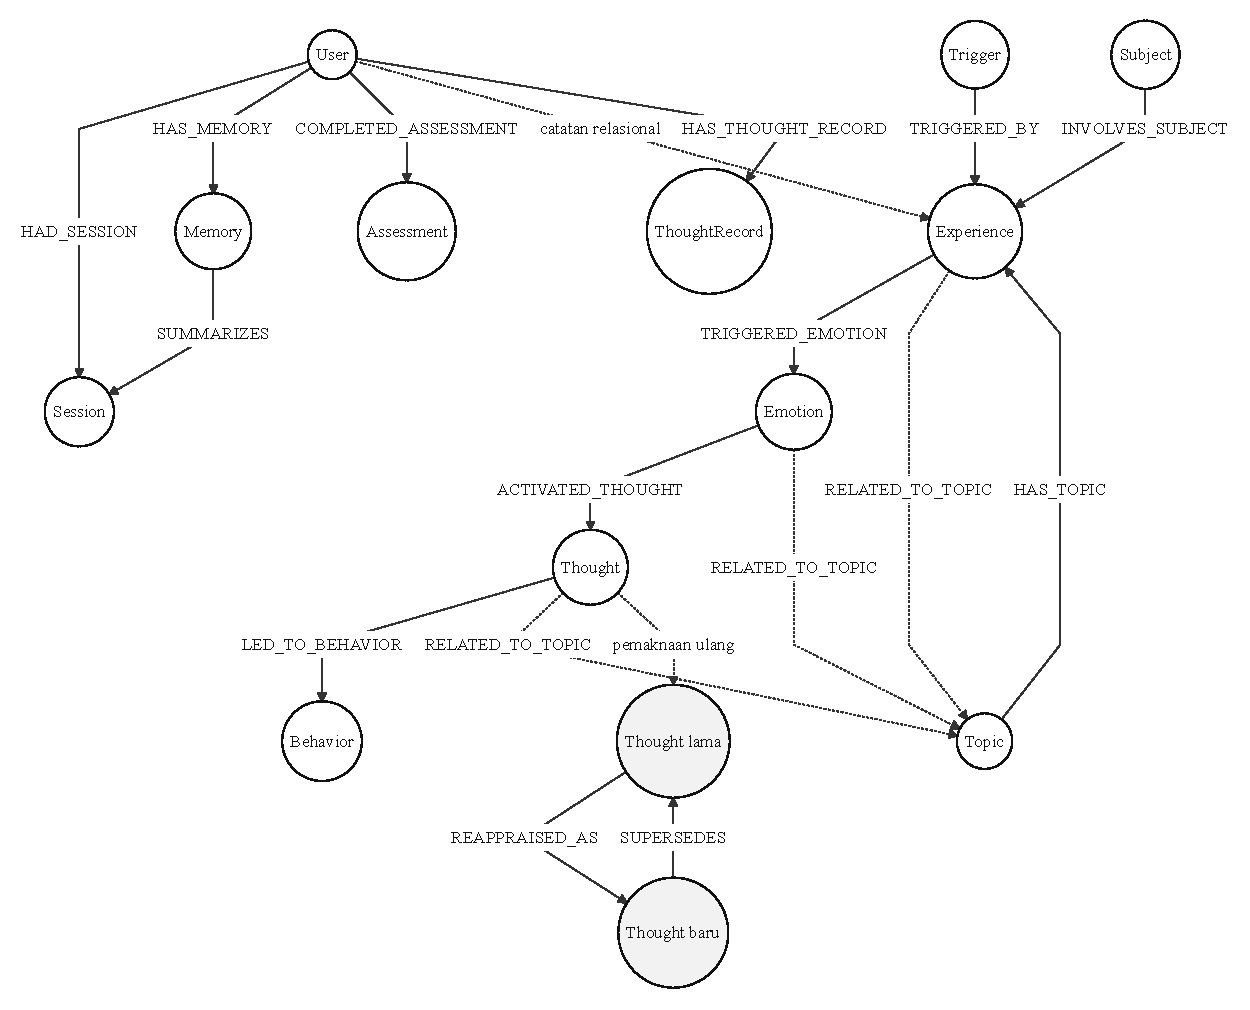
\includegraphics[width=0.95\textwidth]{figures/kg_schema.pdf}
  \caption[Skema implementasi \textit{knowledge graph} afektif]{Skema implementasi \textit{knowledge graph} afektif yang digunakan untuk menyimpan memori relasional pengguna.}
  \label{fig:kg-schema}
\end{figure}

\begin{table}[!htbp]
\centering
\caption{Node dan relasi utama pada memori AXIS}
\label{tab:node-relasi-utama}
{\footnotesize
\begin{tabularx}{\textwidth}{|>{\raggedright\arraybackslash}p{3cm}|>{\raggedright\arraybackslash}X|>{\raggedright\arraybackslash}X|}
\hline
\rowcolor{tableheadgray}
\textbf{Kelompok} & \textbf{Node utama} & \textbf{Contoh relasi} \\
\hline
Konteks percakapan & User, Session, Memory & HAD\_SESSION, HAS\_MEMORY \\
\hline
Model CBT & Experience, Emotion, Thought, ThoughtRecord, Behavior, Trigger & EXPERIENCED, FELT, HAS\_THOUGHT, HAS\_THOUGHT\_RECORD, EXHIBITED, TRIGGERED\_BY \\
\hline
Konteks mahasiswa & Subject, Topic & HAS\_SUBJECT, HAS\_RECURRING\_THEME, INVOLVES\_SUBJECT \\
\hline
Pemantauan & Assessment & COMPLETED\_ASSESSMENT \\
\hline
\textit{Lifecycle} & Thought, Experience, Trigger, Behavior & SUPERSEDES, REAPPRAISED\_AS, UPDATE relasi aktif/tidak aktif \\
\hline
\end{tabularx}
}
\end{table}

Penulisan memori dilakukan setelah sesi tidak aktif. \textit{Session sweeper} menandai sesi yang layak diproses, \textit{finalizer} membaca riwayat percakapan, menyaring pesan PHQ-9 yang bersifat administratif, mengekstrak informasi yang layak disimpan, lalu menulis hasilnya ke Neo4j dan pgvector. Alur ini ditunjukkan pada Gambar \ref{fig:seq-session-finalize}. Mode \textit{Confession Space} dikecualikan dari proses ini sehingga percakapan suara sementara tidak menjadi memori jangka panjang.

Pengaturan \textit{temperature} model bahasa dibedakan menurut sifat tugasnya, bukan diseragamkan. Komponen klasifikasi/penilaian tertutup, seperti \textit{scorer} PHQ-9 dan \textit{judge} EPITOME (Subbab~\ref{sec:evaluasi-komparatif}), memakai \textit{temperature} 0 karena keluarannya berupa label atau skor kategorikal yang menuntut hasil identik untuk masukan identik. Ekstraktor \textit{knowledge graph} dan peringkas sesi memakai \textit{temperature} 1 karena keduanya bukan sekadar mengklasifikasi, melainkan turut menyusun teks bebas (deskripsi Experience, ringkasan Memory) yang secara sengaja dibuat bervariasi agar tidak terasa kaku atau berulang secara mekanis pada memori yang dibaca kembali oleh pengguna. Label dan struktur graf dari pesan yang sama karena itu tidak dijamin identik pada dua kali proses berbeda. Kebutuhan N-01 pada Lampiran~\ref{lamp:fr} dibatasi pada \textit{audit trail guardrail}, yaitu keterlacakan jejak keputusan node dan cabang keselamatan, bukan reproduksibilitas persis ekstraksi graf. \textit{Trade-off} determinisme lawan kealamian bahasa ini belum diuji secara terukur (mis. menjalankan pesan yang sama berulang kali dan mengukur variasi label yang dihasilkan)\ifdefined\seminarhasilmode.\else, dan dicatat sebagai keterbatasan metodologis pada Keterbatasan BAB V (Subbab~\ref{sec:keterbatasan}).\fi

\begin{figure}[!htbp]
  \centering
  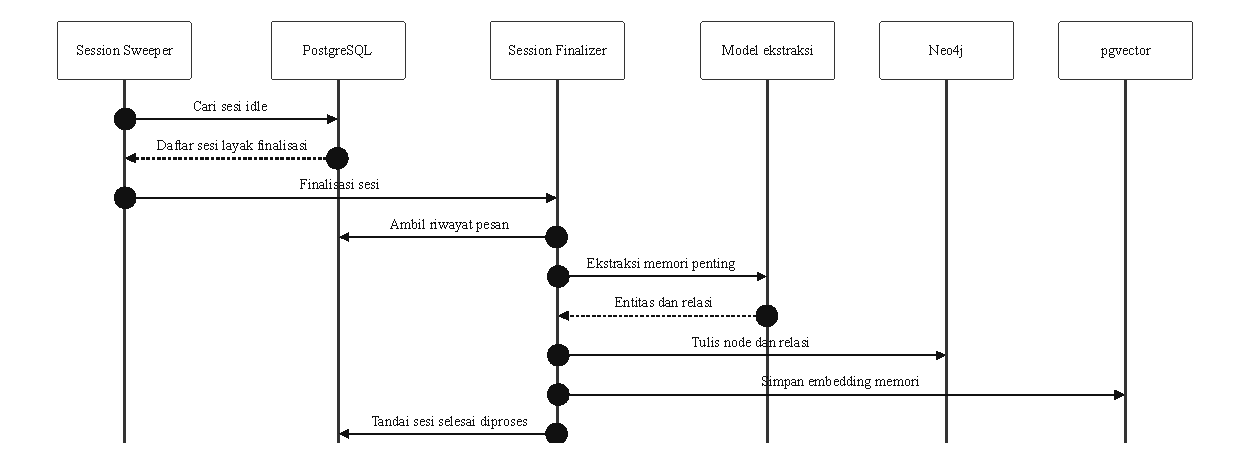
\includegraphics[width=0.95\textwidth]{figures/seq_session_finalize.pdf}
  \caption[Finalisasi sesi oleh proses \textit{session sweep}]{Alur finalisasi sesi asinkron untuk menulis memori lintas sesi ke Neo4j dan pgvector.}
  \label{fig:seq-session-finalize}
\end{figure}

Integrasi Neo4j dan pgvector tidak menggunakan \textit{distributed transaction}. Strategi yang diimplementasikan lebih sederhana dan sesuai kebutuhan purwarupa: Neo4j diperlakukan sebagai sumber utama, sementara pgvector adalah cermin semantik yang dapat dibuat ulang. Setiap node yang dapat dicari secara semantik membawa penanda sinkronisasi vektor. Ketika penulisan ke pgvector berhasil, sistem mencoba menandai node sebagai tersinkron. Jika pembalikan \textit{flag} gagal atau \textit{embedding} belum tersedia, node tetap dapat diproses ulang oleh penyapu sinkronisasi berikutnya. Operasi \textit{upsert} pgvector dibuat idempoten melalui kunci identitas node graf, sehingga percobaan ulang tidak membuat duplikasi. Pendekatan ini tidak sekuat transaksi terdistribusi, tetapi cukup untuk menjaga konsistensi eventual pada arsitektur hibrid yang memisahkan graf relasional dan pencarian semantik.

\textit{Lifecycle} memori diimplementasikan agar memori dapat berubah. Pikiran lama dapat digantikan oleh pikiran baru, pengalaman dapat ditafsirkan ulang, trigger dapat dinonaktifkan, dan memori yang menua dapat kehilangan kepentingannya. Alur \textit{lifecycle} tersebut ditunjukkan pada Gambar \ref{fig:kg-lifecycle}.

\begin{figure}[!htbp]
  \centering
  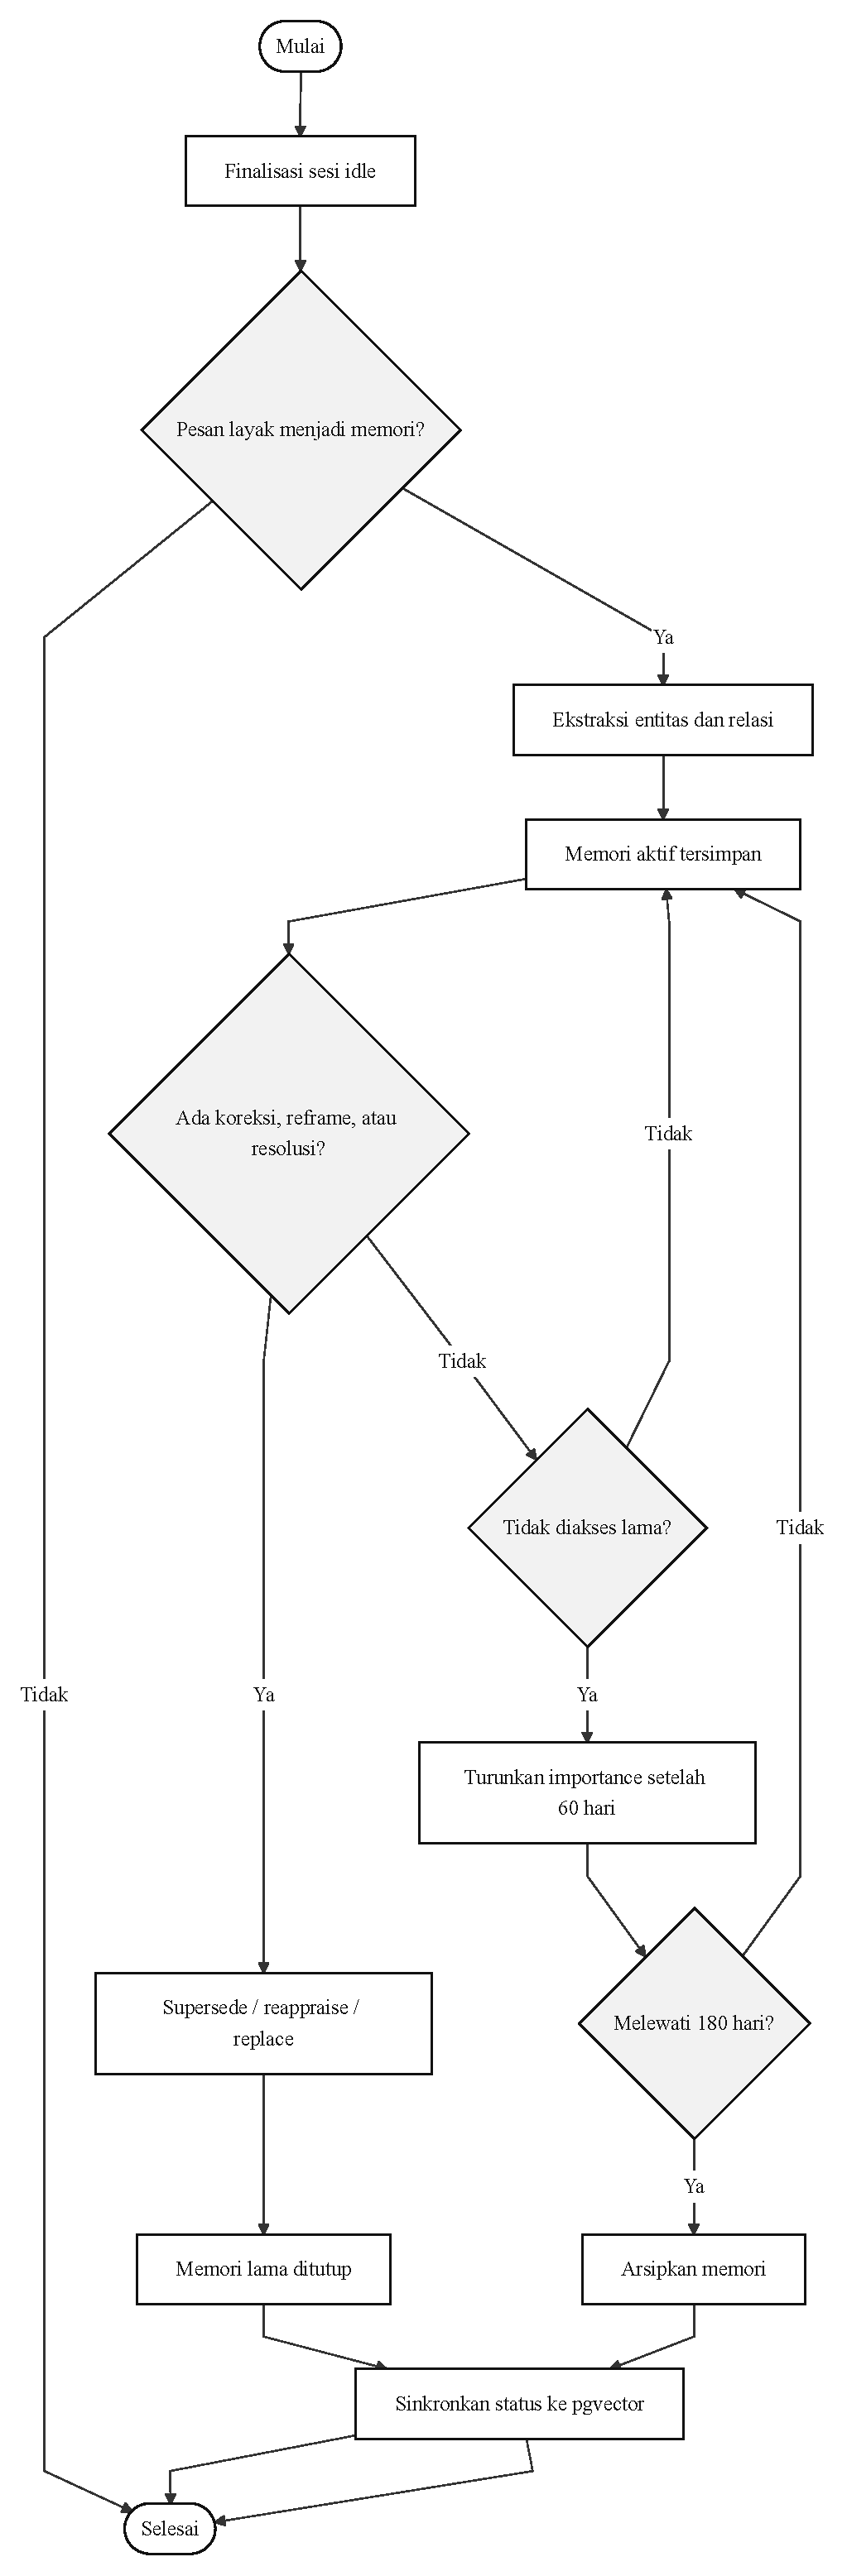
\includegraphics[width=0.95\textwidth,height=0.88\textheight,keepaspectratio]{figures/kg_lifecycle.pdf}
  \caption[Implementasi pembaruan siklus hidup memori]{Implementasi pembaruan siklus hidup memori pada \textit{knowledge graph}, termasuk supersesi, reappraisal, dan penonaktifan memori.}
  \label{fig:kg-lifecycle}
\end{figure}

Perilaku operasi \textit{lifecycle} ini pada percakapan lintas sesi yang sesungguhnya (bukan hanya pengujian unit terhadap objek masukan yang disusun manual) diverifikasi dan dilaporkan pada Subbab~\ref{sec:evaluasi-fungsional}.

Pada saat respons dibuat, AXIS tidak memasukkan seluruh memori ke dalam \textit{prompt}. \textit{Context builder} mengambil kandidat dari beberapa jalur, yaitu pencarian semantik pgvector, sinyal graf terfokus (selanjutnya disebut \textit{focused recall}), tema berulang, subjek penting, dan konteks keselamatan. Kandidat tersebut kemudian digabungkan melalui \textit{reciprocal rank fusion} (RRF), dinilai ulang oleh \textit{graph reranker}, lalu dipilih dengan \textit{maximal marginal relevance} (MMR) agar konteks tidak penuh oleh informasi yang saling mengulang. Ketiga tahap ini diformulasikan secara eksplisit di bawah agar dapat diimplementasikan ulang tanpa membaca kode sumber.

\textit{Tahap 1: RRF.} Setiap kandidat memori $d$ muncul pada satu atau lebih daftar terurut $r$ (pencarian semantik memori dan pengalaman). Skor fusi dihitung sebagai

\begin{equation}
\mathrm{RRF}(d) = \sum_{r \in R} \frac{1}{k + \mathrm{rank}_r(d)}, \qquad k = 60
\label{eq:rrf}
\end{equation}

dengan $\mathrm{rank}_r(d)$ adalah posisi $d$ pada daftar $r$ (mulai dari 1), dan $k=60$ adalah konstanta peredam standar pada literatur RRF \parencite{cormack2009rrf} yang mengurangi pengaruh peringkat teratas tunggal.

\textit{Tahap 2: \textit{graph reranker}.} Skor akhir tiap kandidat adalah kombinasi linear terbobot:

\begin{equation}
\mathrm{skor}(d) = w_{\mathrm{rrf}} \widehat{\mathrm{RRF}}(d) + w_{\mathrm{imp}} I(d) + w_{\mathrm{rich}} R(d) + w_{\mathrm{rec}} T(d) + w_{\mathrm{safe}} S(d)
\label{eq:rerank}
\end{equation}

dengan bobot $w_{\mathrm{rrf}}=0{,}50$, $w_{\mathrm{imp}}=0{,}15$, $w_{\mathrm{rich}}=0{,}15$, $w_{\mathrm{rec}}=0{,}10$, $w_{\mathrm{safe}}=0{,}10$ (jumlah 1, ditetapkan secara heuristik berdasarkan urutan kepentingan sinyal, bukan hasil \textit{tuning} otomatis pada data berlabel), dan komponen berikut. $\widehat{\mathrm{RRF}}(d)$ adalah skor RRF Persamaan \ref{eq:rrf} dinormalisasi terhadap nilai RRF tertinggi pada batch kandidat. $I(d)$ adalah kepentingan node, dibatasi maksimum 1. $R(d)$ adalah kekayaan relasi, dihitung $0{,}20$ untuk tiap dimensi KG yang terhubung ke kandidat (Subject, Trigger, Emotion, Thought, Behavior), maksimum 1. $T(d)$ adalah skor kebaruan dengan peluruhan eksponensial waktu paruh 30 hari, $T(d) = \exp(-\ln 2 \cdot \mathrm{hari}/30)$. $S(d)$ adalah relevansi keselamatan, disediakan sebagai bidang \textit{reserved} sesuai batasan pada Subbab~\ref{sec:batasan-masalah}; pada implementasi saat ini nilainya selalu 0 karena belum ada sinyal keselamatan konkret yang dihubungkan ke skor kandidat, sehingga bobot $w_{\mathrm{safe}}$ secara efektif tidak berkontribusi pada Persamaan \ref{eq:rerank}.

\textit{Tahap 3: MMR.} Dari kandidat terurut hasil Persamaan \ref{eq:rerank}, MMR memilih $n$ kandidat secara iteratif (kandidat dengan skor MMR tertinggi dipilih pada tiap langkah, lalu dikeluarkan dari kumpulan kandidat) untuk menyeimbangkan relevansi dan keragaman:

\begin{equation}
\mathrm{MMR}(d) = \lambda \cdot \mathrm{skor}(d) - (1-\lambda) \max_{d' \in \mathrm{Selected}} \mathrm{sim}(d, d')
\label{eq:mmr}
\end{equation}

dengan $\lambda = 0{,}70$, $\mathrm{sim}(d,d')$ adalah kemiripan \textit{Jaccard} tingkat kata antara teks dua kandidat, dan $n=5$ pada kondisi normal (naik menjadi 10 ketika pesan pengguna terdeteksi sebagai referensi balik atau permintaan klarifikasi, sehingga \textit{context builder} menggali lebih dalam). Dengan demikian, \textit{fusion ranking} bukan lagi sekadar rencana masa depan, melainkan sudah menjadi bagian dari \textit{context builder} utama, meskipun evaluasi kuantitatif terhadap bobot \textit{ranking}, termasuk pertanyaan apakah bobot heuristik ini sudah optimal dibanding alternatif yang di-\textit{tuning} pada data berlabel, masih perlu diperluas pada penelitian lanjutan. Alur pemilihan konteks ditunjukkan pada Gambar \ref{fig:context-builder-ranking}.

\begin{figure}[!htbp]
  \centering
  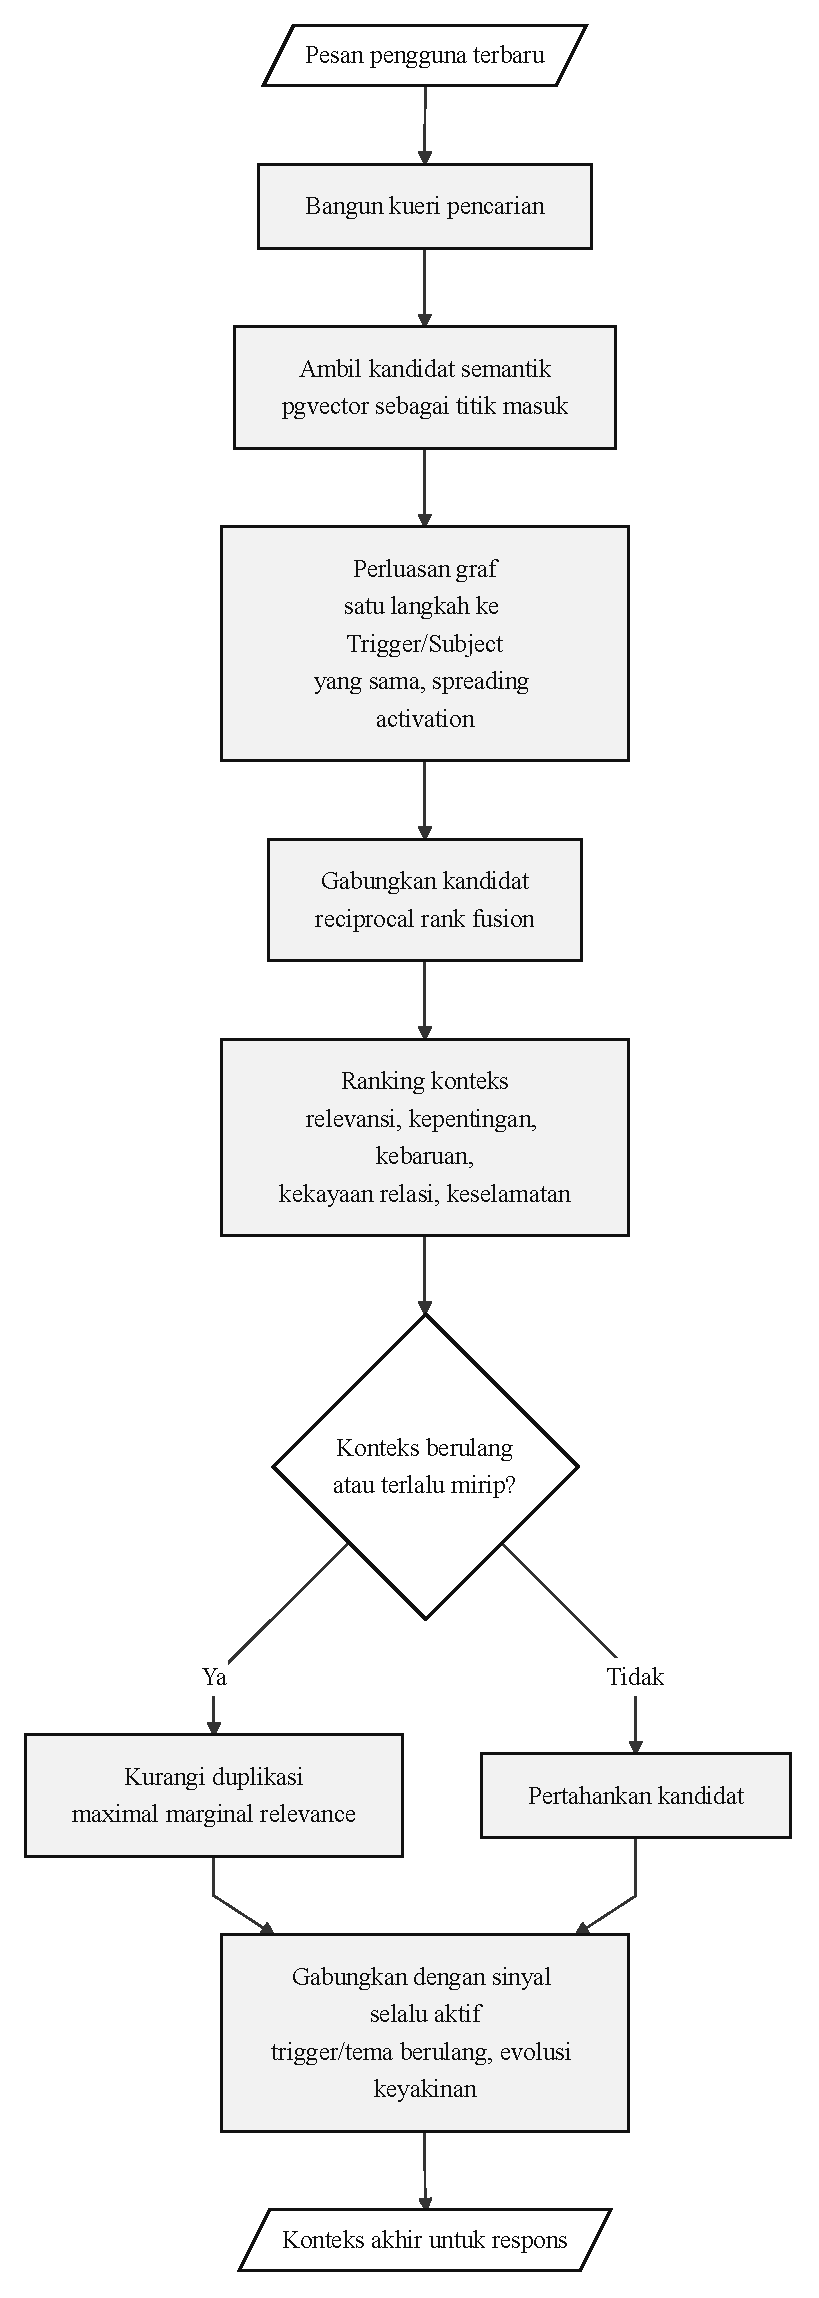
\includegraphics[width=0.9\textwidth,height=0.58\textheight,keepaspectratio]{figures/context_builder_ranking.pdf}
  \caption[Implementasi pemilihan konteks memori]{Implementasi pemilihan konteks memori dari kandidat semantik dan relasional sebelum diberikan kepada pembangkit respons.}
  \label{fig:context-builder-ranking}
\end{figure}

\subsection{Antarmuka dan Kendali Pengguna}
\label{sec:hasil-implementasi}

Antarmuka AXIS disediakan sebagai aplikasi web dengan pengalaman mobile sebagai prioritas. Pembahasan pada bagian ini ditulis dari sudut pandang pengguna: apa yang dapat dilakukan pengguna pada setiap halaman, bukan bagaimana komponen \textit{frontend} dibangun. Setiap halaman ditempatkan sebagai perwujudan rumusan masalah: chat dan voice mendukung percakapan pendamping, mood dan PHQ-9 mendukung refleksi kondisi emosional, sedangkan memori, peta memori, profil, bantuan, dan pengaturan memberi transparansi serta kendali atas pengalaman jangka panjang.

\subsubsection{Autentikasi dan Orientasi}
\label{subsec:impl-auth}

Pengguna memulai dari halaman beranda dan autentikasi. Beranda berperan sebagai pintu orientasi: pengguna melihat ajakan untuk melanjutkan cerita, akses cepat ke chat, suara, memori, dan cek suasana hati, serta informasi singkat bahwa AXIS dikembangkan sebagai tugas akhir. Setelah itu, autentikasi memperkenalkan batas non-klinis dan mengarahkan pengguna untuk masuk atau mendaftar sebelum percakapan dan memori personal disimpan. Selain email dan kata sandi, implementasi juga menyediakan autentikasi Google sebagai pilihan masuk yang lebih cepat. Halaman ketentuan dan privasi disediakan sebagai penjelasan pendukung sebelum pengguna mempercayakan data personalnya kepada sistem. Tampilan autentikasi disajikan pada Lampiran~\ref{lamp:ui-support}.

\subsubsection{Chat, Mood, dan PHQ-9}
\label{subsec:impl-chat}

Halaman chat menjadi ruang utama pengguna bercerita. Pengguna dapat membuka sesi lama, memulai sesi baru, menulis pesan, melihat respons AXIS, dan menjawab \textit{chip} PHQ-9 ketika skrining ditawarkan. Mood harian dapat dipilih melalui antarmuka yang lebih ringan sehingga pengguna tidak harus selalu menjelaskan kondisi emosionalnya dengan kalimat panjang. Tampilan chat ditunjukkan pada Gambar \ref{fig:impl-chat}.

\begin{figure}[!htbp]
  \centering
  
\includegraphics[width=0.95\textwidth,height=0.7\textheight,keepaspectratio]{application/03_chat_main.png}
  \caption[Tampilan antarmuka percakapan AXIS]{Tampilan modul percakapan AXIS dengan daftar sesi, ruang pesan, dan kotak input.}
  \label{fig:impl-chat}
\end{figure}

\subsubsection{\textit{Confession Space} dan Fitur Pendukung}
\label{subsec:impl-fitur-pendukung}
\label{subsec:impl-confession-space}

\textit{Confession Space} memberi pengguna ruang suara sementara. Pengguna berbicara melalui mikrofon, sistem menampilkan transkrip dan subtitle, lalu membalas dengan suara dan teks. Isi pesan dan transkrip tidak ditulis ke riwayat pesan permanen atau memori jangka panjang, sehingga pengguna memperoleh ruang yang lebih ringan untuk bercerita. Batas ini berlaku pada penyimpanan utama AXIS, bukan sebagai jaminan bahwa audio tidak pernah melewati sistem lain: implementasi STT dan TTS dapat meneruskan audio atau teks ke penyedia OpenAI, Gemini, atau ElevenLabs sesuai konfigurasi layanan. Pada saat yang sama, \textit{guardrail} tetap aktif jika muncul sinyal risiko. Secara pengalaman, fitur ini menjadi bentuk kendali atas penggunaan memori, bukan klaim anonimitas menyeluruh. Tampilan \textit{Confession Space} ditunjukkan pada Gambar \ref{fig:impl-voice}.

\begin{figure}[!htbp]
  \centering
  
\includegraphics[width=0.95\textwidth,height=0.7\textheight,keepaspectratio]{application/04_confession_space.png}
  \caption[Tampilan \textit{Confession Space} AXIS]{Tampilan \textit{Confession Space} AXIS yang memusatkan interaksi pada tombol mikrofon dan subtitle percakapan suara.}
  \label{fig:impl-voice}
\end{figure}

Halaman profil dan pengaturan memberi pengguna kendali terhadap nama tampilan, bahasa percakapan, avatar berbasis gender, suara companion, mode respons, reset memori, penghapusan riwayat, unduh data, dan hapus akun. Bahasa yang diatur di sini tidak diperlakukan sebagai fitur i18n antarmuka yang menjadi fokus penelitian, melainkan sebagai preferensi konteks agar AXIS dapat menyesuaikan respons percakapan. Halaman bantuan menjelaskan cara menggunakan chat, latihan reflektif, mood, PHQ-9, memori, \textit{Confession Space}, hotline, dan pengelolaan data. Bagian-bagian ini menjadi payung user agency dalam implementasi: pengguna tidak hanya diajak bercerita, tetapi juga diberi ruang untuk memahami, mengatur, dan menghentikan keterlibatannya dengan sistem. Tampilan profil, pengaturan, dan bantuan disajikan pada Lampiran~\ref{lamp:ui-support}.

\subsubsection{Memori, Peta Memori, dan Hotline}
\label{subsec:impl-memori}

Halaman memori memungkinkan pengguna melihat apa yang diingat AXIS, memilih kategori memori, mencari catatan, menyembunyikan konten sensitif, mengubah memori, atau menghapusnya. Halaman peta memori menampilkan hubungan antarkategori memori secara visual agar pengguna memahami bahwa AXIS tidak hanya menyimpan riwayat chat, tetapi juga hubungan antarcerita. Tampilan peta memori ditunjukkan pada Gambar \ref{fig:impl-kg}, sedangkan tampilan dasbor memori disajikan pada Lampiran~\ref{lamp:ui-support}.

\begin{figure}[!htbp]
  \centering
  
\includegraphics[width=0.95\textwidth,height=0.7\textheight,keepaspectratio]{application/06_knowledge_graph.png}
  \caption[Tampilan visualisasi \textit{knowledge graph}]{Tampilan visualisasi \textit{knowledge graph} personal yang memperlihatkan hubungan antarkategori memori.}
  \label{fig:impl-kg}
\end{figure}

Halaman hotline menyediakan rujukan bantuan yang dapat dibuka langsung oleh pengguna maupun diarahkan dari respons krisis. Tampilan halaman hotline disajikan pada Lampiran~\ref{lamp:ui-support}.

\section{Strategi Evaluasi dan Pemetaan Rancangan}
\label{sec:evaluasi}

Evaluasi dilakukan untuk melihat sejauh mana implementasi AXIS menjawab tiga rumusan masalah. Pada tahap seminar hasil, bukti yang telah tersedia terdiri atas validasi fungsional komponen kritis melalui pengujian unit dan integrasi terbatas, serta studi kasus ilustratif terhadap chatbot \textit{baseline} melalui \textit{evaluation pipeline}. Pengujian pengguna nyata belum diperlakukan sebagai bukti final, melainkan sebagai evaluasi lanjutan yang diperlukan sebelum sistem dapat diklaim matang secara pengalaman pengguna.

Evaluasi bab ini mengikuti tiga jalur yang berbeda sifat buktinya. Evaluasi fungsional (Subbab~\ref{sec:evaluasi-fungsional}) memeriksa komponen kritis dan orkestrasinya melalui skenario terkontrol dengan kriteria lulus/gagal. Evaluasi kualitas percakapan dan memori (Subbab~\ref{sec:evaluasi-komparatif}) membandingkan perilaku AXIS dan \textit{baseline} melalui studi kasus, kuantifikasi EPITOME, serta ablasi, sehingga hasilnya dibaca sebagai bukti indikatif, bukan putusan biner. Evaluasi lanjutan (Subbab~\ref{sec:evaluasi-lanjutan}) disiapkan untuk melengkapi sisi pengalaman pengguna yang belum memiliki data pada tahap seminar hasil.

Keempat fokus pembuktian pada bab ini adalah fungsi komponen kritis, orkestrasi graf keputusan, ketahanan \textit{guardrail} terhadap eufemisme krisis, dan kontribusi memori terhadap kesinambungan percakapan. Evaluasi ini tidak dimaksudkan untuk menyatakan AXIS unggul mutlak atas chatbot AI umum. Tabel~\ref{tab:ringkasan-evaluasi} merangkum bukti yang telah dikumpulkan; status tiap rumusan masalah disintesiskan pada akhir bab.

\begin{table}[!htbp]
\centering
\caption{Ringkasan evaluasi yang telah dilaksanakan}
\label{tab:ringkasan-evaluasi}
{\footnotesize
\begin{tabularx}{\textwidth}{|>{\raggedright\arraybackslash}p{3.2cm}|>{\raggedright\arraybackslash}p{3.0cm}|>{\raggedright\arraybackslash}p{2.6cm}|>{\raggedright\arraybackslash}X|}
\hline
\rowcolor{tableheadgray}
\textbf{Evaluasi} & \textbf{Metode Ringkas} & \textbf{Metrik Utama} & \textbf{Hasil Ringkas} \\
\hline
Validasi fungsional komponen kritis & \textit{Test suite} otomatis Python/Go & Persentase \textit{test} lulus & 59/59 \textit{guardrail}, 48/48 CBT, 24/24 PHQ-9 lulus \\
\hline
Benchmark adversarial eufemisme krisis & 19 kalimat krisis tersamar di luar leksikon sistem & Tingkat tangkap & 14/19 (74\%) pada konfigurasi saat ini \\
\hline
Probe \textit{retrieval} Recall@5 & 15 kueri parafrase, tiga pengguna uji & \textit{Recall@5} & 15/15 (100\%) \\
\hline
Validasi cakupan graf keputusan & 9 skenario terkontrol pada graf sesungguhnya & \textit{Node}/cabang tereksekusi & 18/18 \textit{node}, 18/19 cabang (1 cabang secara desain tidak pernah tereksekusi) \\
\hline
Studi kasus ilustratif dan kuantifikasi EPITOME & Transkrip bebas-improvisasi, persona Arya/Budi, dirata-ratakan lintas pengulangan & Skor ER/IP/EX & \textit{Baseline} lebih tinggi pada persona \textit{cold-start}; AXIS setara atau lebih tinggi pada ER/IP persona memori kaya, \textit{baseline} tetap lebih tinggi pada EX \\
\hline
Evaluasi terkontrol \textit{scripted persona} & Giliran pengguna identik pada AXIS dan \textit{baseline} & Latensi, panjang respons & AXIS 5,4--6,2 detik, lebih lambat dari \textit{baseline} \\
\hline
Studi ablasi \textit{retrieval} graf & Graf aktif dibanding nonaktif, tiga persona independen & Skor EPITOME terisolasi & Graf tidak terbukti meningkatkan skor empati \\
\hline
\end{tabularx}
}
\end{table}


\section{Evaluasi Fungsional}
\label{sec:evaluasi-fungsional}

\subsection{Validasi Komponen Kritis}

\subsubsection{Metode Validasi Komponen Kritis}

Evaluasi ini menjadi bukti bagi RM1 (\textit{guardrail} berlapis), RM2 (transisi PHQ-9), dan RM3 (penyimpanan dan pengambilan memori) sekaligus, karena komponen kritis yang divalidasi mencakup ketiganya. Validasi fungsional dilakukan pada bagian-bagian yang paling menentukan konsistensi rancangan: penyaringan pesan PHQ-9 sebelum finalisasi memori, eskalasi PHQ-9 item ke-9, \textit{guardrail} berlapis, serta alur penyimpanan dan pengambilan memori (termasuk pengecualian sesi \textit{Confession Space} dari penulisan memori). Repositori saat ini memuat 54 file pengujian Python dan Go yang mencakup layanan agentik dan \textit{backend}.

\subsubsection{Hasil Validasi Komponen Kritis}

Ringkasan validasi disajikan pada Tabel \ref{tab:evaluasi-fungsional}.

\begin{table}[!htbp]
\centering
\caption{Status validasi fungsional komponen kritis sistem}
\label{tab:evaluasi-fungsional}
{\footnotesize
\begin{tabularx}{\textwidth}{|>{\raggedright\arraybackslash}p{3.0cm}|>{\raggedright\arraybackslash}X|>{\raggedright\arraybackslash}p{3.4cm}|}
\hline
\rowcolor{tableheadgray}
\textbf{Aspek} & \textbf{Kriteria yang diperiksa} & \textbf{Bukti pengujian} \\
\hline
Ekstraksi memori & Cerita pengguna disaring sebelum ditulis sebagai pengalaman, emosi, pikiran, perilaku, subjek, dan topik. Pesan administratif PHQ-9 tidak boleh ikut menjadi pengalaman hidup, dan sesi \textit{Confession Space} dikecualikan sepenuhnya dari penulisan memori. & Uji finalisasi sesi dan gerbang penulisan memori. \\
\hline
\textit{Retrieval} memori & Sistem mengambil konteks dari kandidat semantik dan relasional, lalu memilih konteks melalui ranking agar prompt tidak penuh oleh memori berulang. & Uji pembentukan konteks, penjagaan isi memori, dan studi kasus Budi. \\
\hline
\textit{Lifecycle} memori & Memori lama dapat digantikan, ditafsirkan ulang, atau dinonaktifkan melalui operasi \textit{lifecycle}. & Uji penulisan graf, pembaruan status, peluruhan, dan penghapusan. \\
\hline
PHQ-9 & Tawaran, pengisian, penyelesaian, penyimpanan \textit{assessment}, dan eskalasi item risiko berjalan sesuai state. & Uji transisi keadaan, penilaian skor, dan penyampaian percakapan. \\
\hline
Kebijakan dialog CBT & Teknik reflektif hanya dipilih setelah giliran minimum dan muatan emosi memadai, penolakan berturut-turut menekan tawaran teknik baru, dan latihan reflektif tidak diam-diam berlanjut setelah giliran krisis. & Uji pemilihan teknik, gerbang giliran, ambang keyakinan, dan reset pasca-krisis. \\
\hline
\textit{Guardrail} & Risiko eksplisit dan implisit diarahkan ke respons aman tanpa mengganggu percakapan normal. & Uji empat lapis keselamatan dan kontrol akses. \\
\hline
\end{tabularx}
}
\end{table}

Hasil utama dari validasi ini adalah bahwa komponen kritis sudah memiliki bukti fungsional yang dapat ditelusuri. Pengujian \textit{guardrail} lulus pada 59 dari 59 skenario, mencakup sinyal krisis eksplisit, indikasi implisit, penundaan saat PHQ-9 berjalan, dan pesan netral yang tidak boleh salah diklasifikasikan. Pengujian kebijakan dialog CBT juga lulus pada 48 dari 48 skenario, termasuk gerbang giliran minimum, ambang keyakinan per teknik, penolakan teknik berturut-turut, dan reset status setelah jalur krisis. Pengujian PHQ-9 lulus pada 24 dari 24 skenario yang mencakup penawaran, penerimaan atau penolakan, pengisian item, klarifikasi jawaban, penyelesaian skor, serta \textit{routing} setelah \textit{guardrail} dan kebijakan dialog aktif. Di luar angka lulus/gagal tersebut, skenario terarah menunjukkan tiga perilaku penting: teknik \textit{grounding} dapat diikuti \textit{reframing} ketika distorsi kognitif masih relevan, pembatasan penyebutan nama mencegah sapaan terasa berlebihan, dan operasi \textit{lifecycle} memori dapat menandai pikiran lama sebagai tidak aktif ketika pengguna merevisinya pada sesi berikutnya. Rincian skenario, keluaran graf, dan contoh respons ditempatkan pada lampiran.

\subsubsection{Analisis Hasil Validasi Komponen Kritis}

Pengujian tersebut menunjukkan bahwa bagian inti sistem sudah memiliki bukti implementasi. Meski demikian, cakupan ini masih bersifat komponen dan skenario terarah, tidak menggantikan evaluasi pengguna nyata. Skenario \textit{guardrail} yang sudah lulus menguji kata kunci dan frasa yang sudah dikenal sistem, sehingga belum membuktikan seberapa baik \textit{guardrail} menangkap ungkapan krisis yang disamarkan, ungkapan yang justru lebih realistis muncul dari mahasiswa yang enggan menyatakan niatnya secara langsung. Celah ini diuji lebih lanjut lewat benchmark adversarial berikut.

\subsection{Benchmark Adversarial Eufemisme Krisis}

\subsubsection{Metode Benchmark Adversarial Eufemisme Krisis}

Evaluasi ini menjadi bukti bagi RM1, khususnya bagian "aman" pada tuntutan percakapan pendamping. Disusun 19 kalimat adversarial yang menyatakan ide bunuh diri secara implisit tanpa memakai satu pun kata kunci atau frasa yang sudah dikenal sistem (Lampiran~\ref{lamp:adversarial-benchmark}), dijalankan lewat mekanisme deteksi \textit{guardrail} yang sesungguhnya.

\subsubsection{Hasil Benchmark Adversarial Eufemisme Krisis}

Pada konfigurasi \textit{guardrail} yang digunakan saat ini, 14 dari 19 kalimat krisis tersamar terdeteksi (74\%). Dari 18 keluhan sehari-hari sebagai pembanding, satu kalimat salah ditandai sebagai krisis. Daftar kalimat dan keluaran per kasus disajikan pada Lampiran~\ref{lamp:adversarial-benchmark}.

\subsubsection{Analisis Hasil Benchmark Adversarial}

Lima kalimat yang masih lolos menunjukkan bahwa deteksi berbasis frasa acuan belum cukup untuk menangkap seluruh variasi eufemisme. Hasil ini mendukung keberadaan lapisan keselamatan, tetapi belum membenarkan klaim bahwa sistem aman terhadap semua bentuk ungkapan krisis.

Kalibrasi domain mahasiswa pada memori juga diuji secara \textit{end-to-end} melalui beberapa percakapan yang mencakup tekanan akademik, keluarga, organisasi, identitas diri, transisi karier, dan relasi kampus. Hasilnya menunjukkan bahwa jalur penulisan memori, ringkasan sesi, dan pembangkitan respons memakai kerangka domain yang sama: sistem dapat membedakan peran seperti dosen pembimbing dan dosen wali, menulis topik kampus yang relevan, lalu mengambil kembali konteks tersebut pada sesi lanjutan. Namun bukti ini masih berupa kasus terarah, bukan pengukuran presisi/\textit{recall} lintas banyak kueri. Untuk menutup celah tersebut, dijalankan pengujian tambahan bergaya \textit{Recall@k}.

\subsection{Probe \textit{Retrieval} Recall@5}

\subsubsection{Metode Probe \textit{Retrieval} Recall@5}

Evaluasi ini menjadi bukti bagi RM3, khususnya kemampuan memori jangka panjang mengambil kembali fakta yang relevan lintas sesi. Sebagaimana lazim dipakai pada evaluasi memori percakapan jangka panjang \parencite{maharana2024locomo}, lima belas fakta domain kampus yang berbeda, tersebar pada tiga pengguna uji independen (lima fakta per pengguna, mencakup keenam domain kalibrasi pada Subbab~\ref{sec:batasan-masalah} dengan skenario spesifik yang berbeda per pengguna agar probe menguji generalisasi dan bukan menghafal satu narasi) ditulis ke graf lewat sesi awal masing-masing, kemudian pada sesi baru diajukan kueri susulan yang sengaja diparafrasekan, bukan mengulang kata kunci dari fakta aslinya, agar retrieval yang cocok benar-benar berbasis makna dan bukan pencocokan literal. Setiap kueri dianggap berhasil (\textit{hit}) apabila konteks yang dikembalikan \textit{context builder} pada mekanisme \textit{focused recall} memuat fakta terkait dalam lima kandidat teratas ($k=5$).

\subsubsection{Hasil Probe \textit{Retrieval} Recall@5}

Tabel~\ref{tab:retrieval-recall-summary} merangkum hasil per pengguna; daftar lengkap pasangan fakta dan kueri parafrase tersedia pada Lampiran~\ref{lamp:eval-retrieval}.

\begin{table}[!htbp]
\centering
\caption{Ringkasan probe \textit{retrieval} Recall@5 per pengguna}
\label{tab:retrieval-recall-summary}
{\footnotesize
\begin{tabularx}{\textwidth}{|>{\centering\arraybackslash}p{1.7cm}|>{\centering\arraybackslash}p{2.3cm}|>{\centering\arraybackslash}p{3.4cm}|>{\centering\arraybackslash}X|}
\hline
\rowcolor{tableheadgray}
\textbf{Pengguna} & \textbf{Jumlah kueri} & \textbf{Rentang kesamaan} & \textbf{\textit{Hit} Recall@5} \\
\hline
A & 5 & 0,67--0,77 & 5/5 \\
\hline
B & 5 & 0,64--0,75 & 5/5 \\
\hline
C & 5 & 0,84--0,89 & 5/5 \\
\hline
\textbf{Total} & \textbf{15} & \textbf{0,64--0,89} & \textbf{15/15 (100\%)} \\
\hline
\end{tabularx}
}
\end{table}

\subsubsection{Analisis Hasil Probe Recall@5}

Probe ini hanya memuat 15 kueri pada tiga pengguna uji. Nilai 100\% karena itu membuktikan jalur \textit{retrieval} bekerja pada kasus terarah yang mencakup domain kalibrasi, bukan estimasi \textit{recall} populasi. Kueri dengan kesamaan terendah tetap menjadi \textit{hit}, yang memberi indikasi bahwa kecocokan tidak hanya bergantung pada tumpang tindih kata.

\subsection{Cakupan Graf Keputusan}
\label{sec:evaluasi-graf}

\subsubsection{Metode Validasi Cakupan Graf Keputusan}

Evaluasi ini menjadi bukti bagi RM1 (jalur \textit{guardrail} dan krisis), RM2 (alur PHQ-9), dan RM3 (orkestrasi pengambilan memori) sekaligus, karena graf keputusan menyatukan ketiga jalur tersebut dalam satu orkestrasi. Subbab sebelumnya membuktikan bahwa setiap komponen bekerja benar secara tersendiri. Pertanyaan yang belum terjawab adalah apakah orkestrasi antarkomponen, yaitu keputusan node mana yang dijalankan berikutnya untuk kondisi percakapan tertentu, benar-benar mengikuti rancangan. AXIS mengorkestrasikan seluruh node melalui satu graf keputusan (Subbab~\ref{subsec:impl-pipeline-agentik}). Graf ini secara rancangan memiliki 18 node dan 8 titik percabangan yang bersama-sama membentuk 19 kemungkinan jalur berdasarkan kode kondisional yang dituliskan. Validasi pada subbab ini menjalankan graf yang sesungguhnya (bukan simulasi bebas atau pengujian node terisolasi) untuk sembilan skenario representatif, lalu merekam urutan node yang benar-benar dilalui pada tiap skenario sebagai bukti, bukan sekadar hasil akhir percakapannya. Kesembilan skenario dipilih agar bersama-sama menyentuh seluruh 18 node dan 18 dari 19 kemungkinan cabang.

\subsubsection{Hasil Validasi Cakupan Graf Keputusan}

Satu cabang, yaitu eskalasi langsung dari penilaian PHQ-9 tanpa melalui triase krisis, tidak dapat dieksekusi oleh kode yang berjalan saat ini karena kondisi yang menyalakannya juga selalu menyalakan penanda krisis yang diperiksa lebih dahulu. Dengan demikian, sembilan skenario terkontrol mencakup seluruh 18 node dan 18 dari 19 cabang rancangan; 18 cabang tersebut lulus dengan urutan node yang sesuai. Daftar skenario dan titik keputusan yang diuji disajikan pada Lampiran~\ref{lamp:eval-graph-coverage}.

\subsubsection{Analisis Hasil Cakupan Graf Keputusan}

Perlu ditegaskan bahwa cakupan ini membuktikan setiap node dan cabang yang dapat tereksekusi telah tereksekusi minimal sekali pada kondisi terkontrol, bukan bahwa seluruh kombinasi kondisi yang mungkin terjadi pada penggunaan nyata sudah diuji, karena jumlah kombinasi penuh antar-status percakapan, PHQ-9, dan keselamatan terlalu besar untuk diuji habis pada tahap purwarupa. Validasi ini melengkapi, bukan menggantikan, validasi fungsional per komponen pada Tabel~\ref{tab:evaluasi-fungsional}: yang satu membuktikan tiap bagian bekerja benar sendiri-sendiri, yang ini membuktikan bagian-bagian tersebut disambungkan dengan benar. Di luar validasi pada skenario terkontrol ini, kebutuhan non-fungsional agar tiap keputusan \textit{node} dapat ditelusuri (N-01, detailnya telah ditampilkan pada tabel di Lampiran~\ref{lamp:fr}) juga sudah didukung pada lalu lintas produksi: setiap giliran percakapan mencatat jejak \textit{node} dan cabang yang dilalui ke tabel audit terpisah, sehingga penelusuran keputusan tidak bergantung pada pengujian skenario saja.

\section{Evaluasi Kualitas Percakapan dan Memori}
\label{sec:evaluasi-komparatif}

Keempat subbab berikut menguji RM1 dan RM3 secara bersamaan lewat satu rangkaian bukti yang sengaja disusun menyempit secara bertahap, bukan empat evaluasi paralel yang berdiri sendiri: studi kasus bebas-improvisasi memberi gambaran ilustratif pada eksekusi bebas, kuantifikasi EPITOME mengukur dimensi empatinya secara terpisah, evaluasi \textit{scripted persona} mengontrol giliran pengguna agar kedua sistem menerima masukan yang identik, dan studi ablasi mengisolasi kontribusi \textit{retrieval} graf itu sendiri dari faktor arsitektur lain. Pembaca yang menemukan pengulangan pola pada persona Budi di beberapa subbab dapat membacanya sebagai penguatan bertahap, bukan pengukuran yang sama diulang tanpa tujuan.

\subsection{Studi Kasus Bebas-Improvisasi: Arya dan Budi}

\subsubsection{Metode Studi Kasus Bebas-Improvisasi}

Evaluasi ini mengamati RM1 (kualitas percakapan empatik) dan RM3 (kesinambungan memori lintas sesi) pada dua persona bertopik skripsi. Arya merepresentasikan pengguna baru tanpa riwayat, sedangkan Budi merepresentasikan pengguna lama dengan riwayat bimbingan skripsi. Keduanya menjalani sepuluh giliran percakapan bebas-improvisasi setelah pesan pembuka yang sama. AXIS menggunakan konteks hibrid, sedangkan \textit{baseline} menggunakan pencarian semantik dari sumber memori awal yang setara. Dengan rancangan ini, perbedaan yang diamati terutama terletak pada cara kedua sistem membangun konteks, bukan pada ketersediaan riwayat awal yang berbeda.

Gemini digunakan sebagai simulator pengguna dan pembangkit respons; EPITOME dinilai oleh model penilai terpisah. Konfigurasi model, sampling, \textit{embedding}, batas token, dan kondisi penyemaian dicatat pada Lampiran~\ref{lamp:eval-config}, sedangkan transkrip lengkap tersedia pada Lampiran~\ref{lamp:eval-transcripts}. Studi ini bersifat ilustratif, bukan pembandingan terkontrol: simulator dapat mengubah arah percakapan setelah pesan pembuka dan setiap sistem menerima respons pengguna yang terbentuk dari keluaran sistemnya sendiri. Karena itu, bagian ini hanya digunakan untuk membaca perilaku yang muncul pada eksekusi tersebut, bukan untuk menyimpulkan keunggulan kausal salah satu mekanisme memori.

\subsubsection{Hasil Studi Kasus Bebas-Improvisasi}

Pada skenario Arya, AXIS membangun percakapan melalui eksplorasi bertahap: penyebab konkret revisi yang tak kunjung selesai, pikiran katastrofik seputar kegagalan lulus tepat waktu, hingga keraguan atas kemampuan diri sendiri. Teknik \textit{reframing} muncul begitu pengguna mengutarakan pikiran serba-terburuk secara eksplisit, dan disampaikan sebagai ajakan menimbang ulang, bukan koreksi searah:

\begin{samepage}
\begin{quote}
\footnotesize
\textbf{AXIS, giliran 6:} ``Pasti bikin khawatir banget ya kalau pikiran itu muncul, langsung ke kemungkinan terburuk kalau skripsi nggak kelar dan gagal lulus. Kalau dipikir-pikir lagi, ada nggak sih kemungkinan lain yang bisa terjadi?''
\end{quote}
\end{samepage}

\textit{Baseline} pada Arya tidak memicu teknik CBT formal sepanjang sepuluh giliran; responsnya konsisten berpola validasi lalu ajakan bercerita lebih lanjut, misalnya pada giliran pembuka: ``Aku bisa merasakan kalau kamu sedang pusing sekali ya akhir-akhir ini karena skripsi. [...] Ada apa yang membuatmu merasa begitu pusing dengan skripsi saat ini? Kalau kamu mau cerita, aku siap mendengarkan.'' Pada Budi, perbedaan cara memakai memori terlihat sejak respons pembuka berikut.

\begin{quote}
\footnotesize
\textbf{\textit{Baseline}, Budi giliran 1:} ``Halo juga! Wah, kedengarannya kamu lagi banyak pikiran ya soal skripsi. Boleh cerita lebih lanjut, kira-kira bagian mana dari skripsi yang bikin kamu pusing akhir-akhir ini?''\\
\textbf{AXIS, Budi giliran 1:} ``Aduh, Budi. Kayaknya skripsi itu lagi berat-beratnya ya. Aku ingat kamu juga pernah cerita kesulitan sama dosen pembimbing dan analisis data yang rasanya stagnan. Sekarang yang bikin pusing banget itu bagian apanya?''
\end{quote}

Kutipan tersebut menunjukkan bahwa AXIS memakai konteks lama sebagai pembuka percakapan, sedangkan \textit{baseline} merespons keluhan saat ini tanpa rujukan ke riwayat Budi. Perbedaan ini hanya menunjukkan perilaku kedua sistem pada eksekusi tersebut; penyebabnya belum dapat diisolasi dari mekanisme \textit{retrieval}, kebijakan dialog, dan volume konteks yang berbeda.

Percakapan Budi dengan AXIS pada eksekusi ini menunjukkan kesinambungan tanpa pengulangan kaku: rujukan ke dosen pembimbing dan analisis data hanya muncul pada giliran pembuka untuk mengikat konteks, sedangkan giliran berikutnya mengikuti arah baru yang dibawa pengguna sendiri (revisi yang terasa menumpuk, harapan akan validasi dari dosen pembimbing, hingga upaya tetap bertahan meski lelah), termasuk satu giliran validasi eksternal dari dosen pembimbing yang secara eksplisit ditandai AXIS sebagai kebutuhan inti pengguna. Pola ini menunjukkan bahwa kesinambungan memori dan kepekaan terhadap pergeseran topik dapat berjalan bersamaan, sejalan dengan pengamatan pada skenario Arya di mana teknik reflektif juga hanya dipicu ketika sinyal distorsi kognitif benar-benar muncul, bukan disisipkan begitu saja pada tiap giliran.

Ringkasan pengamatan ditunjukkan pada Tabel \ref{tab:evaluasi-komparatif-hasil}.

\begin{table}[!htbp]
\centering
\caption{Ringkasan studi kasus ilustratif AXIS dan chatbot \textit{baseline} pada dua persona}
\label{tab:evaluasi-komparatif-hasil}
{\footnotesize
\begin{tabularx}{\textwidth}{|>{\raggedright\arraybackslash}p{3.2cm}|>{\raggedright\arraybackslash}X|>{\raggedright\arraybackslash}X|}
\hline
\rowcolor{tableheadgray}
\textbf{Aspek} & \textbf{\textit{Baseline}} & \textbf{AXIS} \\
\hline
Arya, pengguna baru & Validasi dan ajakan bercerita konsisten di seluruh 10 giliran, tidak pernah memicu teknik CBT. & Eksplorasi bertahap, dengan \textit{reframing} dipicu tepat ketika pikiran katastrofik diutarakan secara eksplisit. \\
\hline
Budi, pengguna lama & Tidak menyebut dosen pembimbing/analisis data sama sekali pada eksekusi ini karena topik bergeser ke keluhan yang dibawa pengguna sendiri. & Menyebut dosen pembimbing/analisis data pada giliran ke-1 untuk membuka kesinambungan, lalu mengikuti topik baru yang dibawa pengguna tanpa mengulang rujukan lama. \\
\hline
Perbedaan yang diamati & Pada eksekusi ini, pencarian semantik tidak menyisipkan memori lama ketika topik percakapan bergeser. & Pada eksekusi ini, AXIS menyisipkan rujukan memori lama pada giliran pembuka untuk mengikat kesinambungan cerita. \\
\hline
Risiko respons & Cenderung memberi validasi generik tanpa menggali struktur pikiran pengguna, dan kehilangan akses ke memori lama begitu topik bergeser. & Teknik reflektif tidak selalu menyala meski memori lama tersedia, karena kebijakan dialog menunggu sinyal distorsi atau distres yang cukup kuat. \\
\hline
\end{tabularx}
}
\end{table}

\subsubsection{Analisis Hasil Studi Kasus}

Temuan pada eksekusi ini memberi indikasi yang lebih spesifik dibanding klaim umum ``AXIS lebih baik mengingat''. Pada skenario Budi, \textit{baseline} tidak menyinggung memori lama, sedangkan AXIS memakai rujukan memori pada giliran pembuka lalu mengikuti pergeseran topik tanpa mengulanginya. Perbedaan tersebut menunjukkan cara kedua konfigurasi membangun konteks pada transkrip ini, tetapi belum cukup untuk menetapkan penyebabnya pada satu mekanisme \textit{retrieval}. Kesinambungan konteks juga tidak otomatis menyalakan teknik reflektif: pemilihan teknik pada AXIS tetap menunggu sinyal distorsi kognitif atau distres yang cukup kuat pada kedua persona, bukan aktif pada setiap giliran begitu memori lama tersedia. Pembahasan kritis independen mengenai temuan ini disajikan pada Lampiran~\ref{lamp:eval-critical}.

Perlu ditegaskan satu keterbatasan penting pada perbandingan ini. \textit{Baseline} dan AXIS tidak hanya berbeda pada mekanisme \textit{retrieval} (graf berbanding pencarian semantik murni), tetapi juga pada volume konteks yang diterima: \textit{baseline} menerima ringkasan memori singkat tanpa riwayat percakapan sama sekali, sedangkan AXIS menerima konteks multi-sinyal yang jauh lebih besar beserta riwayat giliran. AXIS juga memiliki lapisan pemrosesan tambahan yang tidak dimiliki \textit{baseline}, yaitu kebijakan dialog CBT dan \textit{guardrail} berlapis. Perilaku ``menyisipkan rujukan memori lama secara proaktif pada giliran pembuka'' yang diamati pada AXIS karenanya tidak dapat dipastikan berasal dari penalaran graf itu sendiri. Perilaku yang sama secara teoretis dapat pula dihasilkan oleh kebijakan dialog yang menentukan kapan sebuah konteks layak disisipkan, terlepas dari representasi memorinya berbentuk graf atau vektor. Studi kasus ini dengan demikian mendukung klaim bahwa AXIS \emph{secara keseluruhan} berperilaku berbeda dari \textit{baseline}, tetapi tidak dapat mengisolasi \textit{knowledge graph} sebagai satu-satunya penyebab perbedaan tersebut, konsisten dengan batasan evaluasi kausal pada Subbab~\ref{sec:batasan-masalah}. Keterbatasan ini dicatat sebagai batas pembacaan hasil, bukan sebagai klaim final bahwa satu komponen memori sudah terbukti paling menentukan.

\subsection{Kuantifikasi dengan EPITOME}

\subsubsection{Metode Kuantifikasi EPITOME}

Evaluasi ini menjadi bukti kuantitatif bagi RM1, khususnya dimensi empati yang tidak sepenuhnya tertangkap oleh pengamatan naratif. Pengamatan naratif di atas rentan terhadap bias pembaca, sehingga kualitas respons juga diukur dengan kerangka EPITOME \parencite{sharma2020epitome}, sebuah kerangka penilaian empati berbasis teks yang dikembangkan khusus untuk domain dukungan kesehatan mental daring. EPITOME menilai setiap giliran asisten pada tiga dimensi komunikasi empati, masing-masing berskala 0 sampai 2: \textit{Emotional Reaction} (ER, ekspresi kehangatan atau kepedulian terhadap perasaan pengguna), \textit{Interpretation} (IP, pemahaman tersirat terhadap penyebab perasaan tersebut), dan \textit{Exploration} (EX, upaya menggali hal yang belum diungkapkan pengguna). Karena AXIS dan \textit{baseline} pada penelitian ini adalah sistem generatif dan bukan korpus terklasifikasi seperti pada studi asli EPITOME, penilaian ketiga dimensi dilakukan melalui \textit{LLM-as-judge} dengan \textit{prompt chain-of-thought} terpisah per dimensi, mengikuti metodologi G-Eval \parencite{liu2023geval} untuk penilaian teks generatif dengan LLM. Model \textbf{\textit{gpt-4o}} digunakan sebagai \textit{judge} dengan \textit{temperature} 0 agar penilaian konsisten antar giliran. \textit{Prompt} lengkap ketiga dimensi disertakan pada Lampiran~\ref{lamp:agentic-prompts-epitome}.

Karena simulator pengguna bersifat stokastik, satu transkrip tunggal per sistem per persona rentan terhadap kebetulan arah percakapan pada eksekusi tersebut. Untuk mengurangi kerentanan ini, kuantifikasi EPITOME pada laporan ini dijalankan pada beberapa pengulangan independen per persona per sistem (tiga pengulangan untuk Arya, dua pengulangan untuk Budi), dengan jumlah pengulangan yang disamakan antara AXIS dan \textit{baseline} agar perbandingan adil. Setiap giliran asisten pada seluruh transkrip dinilai dengan turut menyertakan riwayat percakapan sebelumnya sebagai konteks bagi \textit{judge}, lalu skor dirata-ratakan lintas pengulangan per sistem per persona.

\subsubsection{Hasil Kuantifikasi EPITOME}

Hasil rata-rata per sistem per persona divisualisasikan pada Gambar \ref{fig:epitome-chart}: \textit{baseline} mencatat ER 1,90, IP 1,93, dan EX 2,00 pada Arya, serta ER 1,80, IP 1,95, dan EX 2,00 pada Budi, sedangkan AXIS mencatat ER 1,70, IP 1,83, dan EX 1,60 pada Arya, serta ER 1,90, IP 1,90, dan EX 1,70 pada Budi.

\begin{figure}[!htbp]
\centering
\begin{tikzpicture}
\begin{axis}[
    ybar,
    bar width=8pt,
    width=0.85\textwidth,
    height=6.5cm,
    ymin=0, ymax=2.3,
    ylabel={Skor EPITOME (0--2)},
    symbolic x coords={ER, IP, EX},
    xtick=data,
    enlarge x limits=0.25,
    legend style={at={(0.5,-0.18)}, anchor=north, legend columns=-1, font=\footnotesize},
    nodes near coords,
    every node near coord/.append style={font=\tiny},
    ymajorgrids=true,
    grid style={gray!25},
]
\addplot[fill=gray!35] coordinates {(ER,1.90) (IP,1.93) (EX,2.00)};
\addplot[fill=gray!70] coordinates {(ER,1.70) (IP,1.83) (EX,1.60)};
\addplot[fill=black!45,postaction={pattern=north east lines}] coordinates {(ER,1.80) (IP,1.95) (EX,2.00)};
\addplot[fill=black!80,postaction={pattern=north east lines}] coordinates {(ER,1.90) (IP,1.90) (EX,1.70)};
\legend{\textit{Baseline}\ Arya, AXIS Arya, \textit{Baseline}\ Budi, AXIS Budi}
\end{axis}
\end{tikzpicture}
\caption{Perbandingan skor EPITOME AXIS dan \textit{baseline} per dimensi, dirata-ratakan lintas pengulangan}
\label{fig:epitome-chart}
\end{figure}

\subsubsection{Analisis Hasil Kuantifikasi EPITOME}

Gambar~\ref{fig:epitome-chart} menunjukkan pola yang berbeda antara kedua persona. Pada Arya (\textit{cold-start}, tanpa memori lama sama sekali), \textit{baseline} unggul pada ketiga dimensi. Tanpa memori yang perlu diintegrasikan, \textit{baseline} secara konsisten memvalidasi lalu menggali lebih lanjut pada hampir setiap giliran, pola yang selaras langsung dengan definisi ketiga dimensi EPITOME. Pada Budi (memori kaya), pola berbalik pada dua dari tiga dimensi: AXIS sedikit lebih tinggi pada ER dan setara pada IP, sementara \textit{baseline} masih unggul pada EX.

Pemeriksaan giliran berskor rendah pada EX menunjukkan pola yang konsisten pada AXIS: sebagian giliran menutup respons dengan pernyataan reflektif yang menegaskan kembali perasaan yang sudah diutarakan pengguna, alih-alih membuka sisi yang belum terucap. Pernyataan seperti ini tergolong kuat pada Interpretation, tetapi tidak otomatis terhitung sebagai Exploration menurut definisi dimensi tersebut, karena Exploration secara spesifik menilai upaya menggali hal yang \emph{belum} diungkapkan. Pola ini konsisten dengan rancangan AXIS yang sengaja tidak selalu menutup respons dengan pertanyaan penggali (lihat mekanisme variasi ritme giliran, Subbab~\ref{subsec:impl-pipeline-agentik}), sehingga skor EX yang lebih rendah sebagian mencerminkan pilihan rancangan itu sendiri, bukan semata kekurangan kemampuan menggali.

Untuk RM1, hasil tersebut tidak mendukung klaim bahwa AXIS lebih empatik daripada \textit{baseline} pada ukuran EPITOME. Bukti percakapan yang bermakna dan aman perlu dibaca terpisah: studi kasus menunjukkan penggunaan konteks lama oleh AXIS pada eksekusi tertentu, sedangkan keamanan memiliki bukti fungsional \textit{guardrail} dan tingkat tangkap 74\% pada 19 kalimat krisis tersamar. Karena studi ini hanya mencakup dua pasang transkrip bebas-improvisasi, hasilnya belum dapat digeneralisasi; perbandingan berikutnya perlu memakai giliran pengguna terskrip dan penilaian pembanding.

\subsection{Evaluasi Terkontrol dengan \textit{Scripted Persona}}

\subsubsection{Metode Evaluasi \textit{Scripted Persona}}

Evaluasi ini menjadi bukti bagi RM1 (teknik reflektif yang muncul pada persona Arya) dan RM3 (kesinambungan memori serta biaya latensinya pada persona Budi) sekaligus. Sebagai pelengkap, dijalankan juga evaluasi terkontrol lewat \textit{pipeline} evaluasi menggunakan \textit{scripted persona}: berbeda dari \textit{simulated user}, pada \textit{run} ini AXIS dan \textit{baseline} menerima rangkaian pesan pengguna yang sama persis. Dua persona digunakan: Arya sebagai pengguna baru tanpa memori jangka panjang, dan Budi sebagai pengguna lama dengan memori tentang bimbingan skripsi, Bab 3, dosen pembimbing, dan kecemasan akademik. Masing-masing persona menjalankan sepuluh giliran pengguna pada setiap sistem, sehingga setiap transkrip berisi sedikitnya dua puluh pesan pengguna-asisten. Ringkasan eksekusi ditunjukkan pada Tabel~\ref{tab:evaluasi-scripted-persona}.

\begin{table}[!htbp]
\centering
\caption{Ringkasan evaluasi terkontrol berbasis \textit{scripted persona}}
\label{tab:evaluasi-scripted-persona}
{\footnotesize
\setlength{\tabcolsep}{3pt}
\begin{tabularx}{\textwidth}{|>{\raggedright\arraybackslash}p{2.0cm}|>{\raggedright\arraybackslash}p{1.8cm}|>{\raggedright\arraybackslash}p{1.5cm}|>{\centering\arraybackslash}p{0.9cm}|>{\centering\arraybackslash}p{0.9cm}|>{\centering\arraybackslash}p{0.9cm}|>{\centering\arraybackslash}X|}
\hline
\rowcolor{tableheadgray}
\textbf{Persona} & \textbf{Kondisi} & \textbf{Sistem} & \textbf{Turn} & \textbf{Error} & \textbf{Klinis} & \textbf{Rerata latensi} \\
\hline
Arya & \textit{Cold-start} & AXIS & 10 & 0 & 0 & 6229,4 ms \\
\hline
Arya & \textit{Cold-start} & \textit{Baseline} & 10 & 0 & 0 & 3326,7 ms \\
\hline
Budi & \textit{Rich-memory} & AXIS & 10 & 0 & 0 & 5388,2 ms \\
\hline
Budi & \textit{Rich-memory} & \textit{Baseline} & 10 & 0 & 0 & 3871,4 ms \\
\hline
\end{tabularx}
}
\end{table}

\subsubsection{Hasil Evaluasi Persona Arya}

Pada persona Arya, AXIS tidak memiliki memori jangka panjang. Konteks yang masuk ke pembangkit respons memang tercatat pada setiap giliran, tetapi isinya menyatakan bahwa belum ada konteks lama untuk pengguna tersebut dan hanya memuat riwayat percakapan jangka pendek. Hasil ini penting karena mencegah pembacaan yang keliru: kemunculan blok konteks pada pengguna baru tidak berarti sistem sedang mengklaim memiliki memori lintas sesi. Pada percakapan Arya, AXIS menjalankan validasi, \textit{behavior activation}, dan \textit{thought record} ketika pengguna mulai meminta bantuan merapikan pikiran. \textit{Baseline} juga memberi respons yang aman, tetapi tidak memiliki catatan teknik reflektif yang dapat ditelusuri. Rerata panjang respons \textit{baseline} juga lebih besar (56,6 kata) dibanding AXIS (41,7 kata), sehingga respons \textit{baseline} cenderung lebih panjang meskipun tidak selalu lebih terarah.

Rerata latensi pada Tabel \ref{tab:evaluasi-scripted-persona} menunjukkan biaya dari \textit{pipeline} AXIS yang lebih panjang. Pada persona Arya, AXIS memerlukan rata-rata 6.229,4 ms, hampir dua kali \textit{baseline} yang berada pada 3.326,7 ms. Pada persona Budi, AXIS berada pada 5.388,2 ms, sedangkan \textit{baseline} 3.871,4 ms. Perbedaan ini konsisten dengan arsitektur AXIS yang menambahkan pengayaan bahasa, \textit{guardrail}, kebijakan dialog, dan \textit{context builder} sebelum respons akhir dibentuk.

\subsubsection{Analisis Latensi Respons}

Selisih ini tidak boleh dibaca sekadar sebagai catatan teknis \textit{trade-off}, melainkan sebagai biaya pengalaman pengguna yang nyata. Literatur interaksi manusia-komputer klasik menempatkan sekitar satu detik sebagai batas agar alur berpikir pengguna tetap terasa tidak terputus meski jeda mulai disadari \parencite{miller1968responsetime}. Kajian yang lebih baru pada \textit{chatbot} secara spesifik juga menunjukkan bahwa waktu respons berfungsi sebagai isyarat sosial yang memengaruhi persepsi kehadiran lawan bicara dan niat memakai sistem kembali, dengan efek yang berbeda antara pengguna baru dan pengguna berpengalaman \parencite{gnewuch2022responsetime}. Latensi AXIS pada rentang 5,4--6,2 detik berada jauh di atas ambang satu detik tersebut, sehingga jeda yang dialami pengguna pada percakapan yang membahas isi emosional berpotensi terasa sebagai keheningan yang canggung, bukan sekadar keterlambatan teknis yang netral. Karena itu, optimasi latensi perlu menjadi bagian evaluasi lanjutan yang diprioritaskan, terutama sebelum sistem dipakai dalam interaksi suara \textit{real-time} yang jauh lebih sensitif terhadap jeda dibanding teks.

\subsubsection{Hasil Evaluasi Persona Budi}

Pada persona Budi, perbedaan memori lebih terlihat. AXIS menerima konteks jangka panjang berupa pengalaman konsultasi skripsi dengan dosen pembimbing, memori tentang Bab 3 yang buntu, serta \textit{focused recall} dengan kemiripan semantik 0,75 pada giliran pertama. Sistem memakai memori tersebut untuk membuka kesinambungan cerita, lalu mengikuti pergeseran topik ketika pengguna meminta agar percakapan karier \textit{backend} tidak selalu ditarik kembali ke dosen pembimbing. Setelah pergeseran topik, metrik mencatat AXIS hanya menyebut \textit{Bab 3} satu kali, \textit{dosen pembimbing} satu kali, dan tidak lagi menyebut \textit{bimbingan}. \textit{Baseline}, sebaliknya, mengambil istilah lama dari \textit{retrieval} vektor secara konsisten: istilah \textit{Bab 3} muncul 30 kali pada kandidat \textit{retrieval}, \textit{dosen pembimbing} 30 kali, dan \textit{bimbingan} 10 kali. \textit{Baseline} tetap relevan untuk \textit{recall} teks mirip, tetapi belum menunjukkan pemanfaatan relasi pengalaman, pemicu, pikiran, dan perilaku.

\subsubsection{Analisis Kontribusi Memori}

\textit{Run} terkontrol ini memperkuat pembacaan yang lebih hati-hati terhadap kontribusi memori AXIS. Bukti yang tersedia belum cukup untuk menyatakan bahwa \textit{knowledge graph} secara kausal sendirian lebih unggul daripada \textit{retrieval} vektor, karena AXIS dan \textit{baseline} tetap berbeda sebagai sistem lengkap. Namun, \textit{run} ini menunjukkan dua hal yang lebih dapat dipertanggungjawabkan. Pertama, AXIS membedakan kondisi \textit{cold-start} dan \textit{rich-memory} secara benar. Kedua, pada pengguna lama, AXIS dapat membawa kembali konteks lama ketika relevan tanpa menjadikannya pengulangan yang mendominasi seluruh percakapan. Ringkasan \textit{run} ini disajikan pada Lampiran~\ref{lamp:eval-scripted-persona}.

\subsection{Studi Ablasi \textit{Retrieval} Graf}
\label{sec:evaluasi-ablasi}

\subsubsection{Metode Studi Ablasi \textit{Retrieval} Graf}

Evaluasi ini menjadi bukti bagi RM3, secara spesifik mengisolasi kontribusi \textit{knowledge graph} terhadap kualitas memori jangka panjang dari faktor arsitektur lain. Perbandingan pada subbab sebelumnya membandingkan AXIS terhadap \textit{baseline} yang berbeda tidak hanya pada mekanisme \textit{retrieval}, tetapi juga pada volume konteks, riwayat percakapan, dan lapisan \textit{guardrail}/kebijakan dialog sekaligus, sehingga kontribusi \textit{knowledge graph} secara spesifik tidak dapat diisolasi dari perbedaan-perbedaan lain tersebut. Untuk mengisolasi kontribusi itu, dijalankan studi ablasi pada AXIS sendiri, bukan perbandingan lintas sistem: \textit{retrieval} berbasis graf dinonaktifkan sementara seluruh lapisan lain (\textit{guardrail}, kebijakan dialog CBT, volume konteks, model bahasa) tetap identik, memakai parameter konfigurasi yang membatasi jalur pengambilan konteks pada pencarian semantik pgvector saja, tanpa fusi RRF, \textit{graph reranker}, maupun MMR (Persamaan \ref{eq:rrf}--\ref{eq:mmr}) yang biasanya berjalan.

Tiga persona dipakai: Arya sebagai kondisi \textit{cold-start}, Budi sebagai pengguna dengan riwayat skripsi, dan persona ketiga dengan tekanan finansial keluarga. Masing-masing menjalankan sepuluh giliran terskrip pada graf aktif, graf nonaktif, dan \textit{baseline} sebagai titik referensi. Setiap kondisi AXIS dimulai dari keadaan memori awal yang sama, sementara urutan teknik CBT diperiksa agar perbedaan respons tidak berasal dari pemilihan teknik yang berbeda. Protokol reset, urutan kondisi, dan artefak per giliran disajikan pada Lampiran~\ref{lamp:eval-ablation}.

\subsubsection{Hasil Studi Ablasi \textit{Retrieval} Graf}

Secara kualitatif, graf aktif membentuk \textit{focused recall} yang mengikuti perubahan topik, sedangkan kondisi tanpa graf cenderung mengirim jumlah kandidat yang tetap dan sebagian tumpang tindih. Contoh konteks dan artefak per giliran disajikan pada Lampiran~\ref{lamp:eval-ablation}.

Skor EPITOME pada kesembilan transkrip dirangkum pada Tabel~\ref{tab:ablasi-epitome}, memakai metodologi penilaian yang sama dengan Gambar~\ref{fig:epitome-chart} (\textit{prompt chain-of-thought} per dimensi, \textbf{\textit{gpt-4o}} sebagai \textit{judge}, \textit{temperature} 0). Meski dimensi dan \textit{judge}-nya identik, Tabel~\ref{tab:ablasi-epitome} berasal dari \textit{run} yang terpisah dari Gambar~\ref{fig:epitome-chart}: giliran pengguna terskrip dengan protokol reset yang menyamakan keadaan memori awal di ketiga kondisi (bukan simulator bebas-improvisasi yang dirata-ratakan lintas pengulangan), dan memakai persona ketiga di luar Arya/Budi. Skor \textit{baseline} pada kedua tabel karenanya tidak dimaksudkan untuk dibandingkan angka demi angka; keduanya menjawab pertanyaan yang berbeda, yaitu perilaku AXIS pada eksekusi bebas dibanding kontribusi spesifik \textit{retrieval} graf pada kondisi yang dikontrol ketat.

\begin{table}[!htbp]
\centering
\caption{Skor EPITOME (skala 0 sampai 2) pada ablasi \textit{retrieval} graf, tiga persona independen}
\label{tab:ablasi-epitome}
{\footnotesize
\begin{tabularx}{\textwidth}{|>{\raggedright\arraybackslash}X|>{\raggedright\arraybackslash}p{2.0cm}|>{\centering\arraybackslash}p{1.3cm}|>{\centering\arraybackslash}p{1.3cm}|>{\centering\arraybackslash}p{1.3cm}|}
\hline
\rowcolor{tableheadgray}
\textbf{Sistem} & \textbf{Persona} & \textbf{ER} & \textbf{IP} & \textbf{EX} \\
\hline
\textit{Baseline} (\textit{temperature} disamakan) & Arya & 1,90 & 1,90 & 1,60 \\
\hline
AXIS, graf aktif & Arya & 1,60 & 1,70 & 1,70 \\
\hline
AXIS, graf nonaktif & Arya & 1,50 & 1,60 & 1,80 \\
\hline
\textit{Baseline} (\textit{temperature} disamakan) & Budi & 1,50 & 1,90 & 1,90 \\
\hline
AXIS, graf aktif & Budi & 1,20 & 1,50 & 1,70 \\
\hline
AXIS, graf nonaktif & Budi & 1,40 & 1,70 & 1,90 \\
\hline
\textit{Baseline} (\textit{temperature} disamakan) & Persona ketiga & 1,80 & 1,70 & 1,60 \\
\hline
AXIS, graf aktif & Persona ketiga & 1,00 & 1,30 & 1,50 \\
\hline
AXIS, graf nonaktif & Persona ketiga & 1,30 & 1,50 & 1,60 \\
\hline
\end{tabularx}
}
\end{table}

Tabel~\ref{tab:ablasi-epitome} menunjukkan dua pola utama. Pertama, \textit{baseline} setara atau lebih tinggi daripada kedua kondisi AXIS pada ER dan IP untuk ketiga persona. Kedua, graf aktif selalu sedikit lebih rendah daripada graf nonaktif pada EX. Perbedaan lain antarpersona tidak seragam, sehingga tabel dan artefak per giliran pada Lampiran~\ref{lamp:eval-ablation} lebih tepat dibaca sebagai dasar pemeriksaan lanjutan, bukan pola umum.

\subsubsection{Analisis Hasil Ablasi \textit{Retrieval} Graf}

Pemeriksaan terhadap giliran berskor rendah menunjukkan bahwa skor terendah tidak terikat pada kondisi graf aktif atau graf nonaktif, melainkan cenderung muncul ketika kebijakan dialog menyampaikan instruksi teknik CBT tanpa didahului validasi emosi yang cukup. Dengan kata lain, jenis giliran tampak lebih langsung memengaruhi skor ER dan EX dibanding bentuk \textit{retrieval} itu sendiri. Temuan ini penting karena mencegah pembacaan yang terlalu cepat: selisih rata-rata pada Tabel~\ref{tab:ablasi-epitome} tidak dapat langsung diklaim sebagai akibat representasi graf semata.

Studi ablasi menahan lapisan lain tetap sama, sehingga hasilnya lebih tepat untuk menilai kontribusi \textit{retrieval} graf daripada studi kasus AXIS--\textit{baseline}. Konsisten dengan batasan pada Subbab~\ref{sec:batasan-masalah}, pada tiga persona dengan satu pengulangan, graf belum terbukti meningkatkan skor empati EPITOME dan tidak dapat dijadikan dasar untuk klaim kausal. Pemeriksaan giliran menunjukkan bahwa kualitas validasi emosi dan jenis respons CBT tampak lebih berpengaruh terhadap ER dan EX daripada bentuk \textit{retrieval}. Kontribusi graf pada tahap ini lebih layak dibaca pada kesinambungan konteks dan pengendalian pengulangan, bukan sebagai peningkatan empati yang telah terbukti.

\section{Evaluasi Lanjutan yang Direncanakan}
\label{sec:evaluasi-lanjutan}

Evaluasi yang belum dijalankan pada tahap seminar hasil dipisahkan dari hasil utama agar pembaca tidak menyamakannya dengan bukti yang sudah terkumpul. Evaluasi lanjutan yang paling penting adalah pengujian pengguna nyata terbatas, yang disiapkan untuk menjawab sisi pengalaman penggunaan yang belum dapat dibuktikan oleh \textit{test suite}, studi kasus, atau ablasi.

\subsection{Pengujian Pengguna Nyata}
\label{sec:evaluasi-pengguna}

Pengujian pengguna nyata dirancang sebagai evaluasi terbatas pada mahasiswa Indonesia, dengan target minimal 12--14 partisipan dan, bila waktu memungkinkan, mendekati 20 partisipan. Instrumen pada Lampiran~\ref{lamp:userstudy} mencakup SUS, kualitas interaksi, kesinambungan memori, keselamatan, rasa didampingi, dan pertanyaan terbuka. Data akan dibaca secara deskriptif sebagai indikasi pengalaman menggunakan purwarupa, bukan generalisasi populasi atau studi klinis.

\section{Diskusi terhadap Rumusan Masalah}
\label{sec:diskusi-hasil}

Berdasarkan studi kasus ilustratif dan \textit{run} terkontrol pada Subbab~\ref{sec:evaluasi-komparatif}, AXIS menunjukkan indikasi awal nilai pada kesinambungan konteks. Pada pengguna lama, respons dapat membawa kembali memori yang relevan tanpa mengulanginya secara kaku di setiap giliran, sehingga percakapan tidak terasa dimulai dari nol maupun terasa seperti rekaman yang diputar ulang. Bukti yang paling kuat pada tahap ini bukan bahwa \textit{knowledge graph} sendirian lebih unggul daripada vektor, melainkan bahwa sistem lengkap AXIS dapat membedakan kondisi \textit{cold-start} dan \textit{rich-memory}, lalu memakai konteks lama secara lebih selektif dibanding \textit{baseline}. Ketiga subbab berikut menghubungkan temuan ini secara eksplisit ke tiap rumusan masalah.

\subsection{RM1: Percakapan Pendamping yang Empatik, Bermakna, dan Aman}

Untuk rumusan masalah pertama, hasilnya masih parsial. Pada studi kasus ilustratif bebas-improvisasi (Subbab~\ref{sec:evaluasi-komparatif}), EPITOME yang dirata-ratakan lintas pengulangan menunjukkan pola yang berbeda antara kedua kondisi memori: pada persona \textit{cold-start} (Arya), \textit{baseline} unggul pada ketiga dimensi karena responsnya yang konsisten memvalidasi lalu menggali lebih lanjut selaras langsung dengan definisi EPITOME ketika tidak ada memori yang perlu diintegrasikan; pada persona memori kaya (Budi), AXIS sedikit lebih tinggi pada ER dan setara pada IP, sementara \textit{baseline} tetap lebih tinggi pada EX. Pemeriksaan giliran berskor rendah menunjukkan bahwa sebagian skor EX yang lebih rendah pada AXIS berasal dari pilihan rancangan yang sengaja tidak menutup setiap giliran dengan pertanyaan penggali (Subbab~\ref{subsec:impl-pipeline-agentik}), bukan semata kekurangan kemampuan menggali. Pola serupa muncul pada evaluasi terkontrol berbasis \textit{scripted persona} yang menyamakan giliran pengguna di kedua kondisi (Tabel~\ref{tab:evaluasi-scripted-persona}): AXIS menjalankan teknik CBT yang dapat ditelusuri meski responsnya lebih ringkas daripada \textit{baseline}, tanpa itu berarti otomatis lebih baik, karena kualitasnya tetap bergantung pada waktu pemilihan teknik dan kesesuaian pertanyaan lanjutan. Selain itu, sisi bahasa informal, campuran bahasa, dan cara halus mengungkapkan masalah belum diuji dengan pengujian bahasa yang luas. Pengujian tambahan pada skenario obrolan kasual tanpa sinyal distres (Lampiran~\ref{lamp:eval-casual}) juga menunjukkan gaya bertanya reflektif AXIS tetap aktif meski topik pembicaraan sepenuhnya non-emosional, mengindikasikan gaya ini belum cukup membedakan kapan penggalian mendalam benar-benar diperlukan. Dengan demikian, RM1 belum boleh dibaca sebagai tuntas, melainkan sebagai implementasi yang hasilnya masih bercampur: kuat pada kondisi memori kaya, tetapi belum menunjukkan keunggulan yang jelas pada percakapan tanpa riwayat sama sekali.

\subsection{RM2: Pemantauan Kondisi Emosional Berkala dan Terstruktur}

Untuk rumusan masalah kedua, mood harian dan PHQ-9 sudah memiliki dasar implementasi yang lebih stabil, dengan seluruh skenario transisi PHQ-9 lulus sebagaimana dirangkum pada Tabel~\ref{tab:evaluasi-fungsional}. Bukti ini sebagian besar bersifat mekanis (lulus/gagal pada skenario terarah); sebagai ilustrasi bahwa transisinya juga dapat terasa menyatu dengan alur percakapan, bukan tiba-tiba berubah menjadi formulir, kutipan berikut menunjukkan giliran saat pengguna sendiri yang membuka topik pengecekan mood di tengah cerita biasa.

\begin{quote}
\footnotesize
\textbf{Pengguna:} ``Boleh nggak aku coba cek mood pake yang 9 pertanyaan itu? Penasaran aja hasilnya kayak gimana.''\\
\textbf{AXIS:} ``Aku mau ngajak kita ngecek kondisi mood-mu lewat 9 pertanyaan singkat (PHQ-9). Tiap pertanyaan menanyakan seberapa sering kamu merasakan sesuatu dalam dua minggu terakhir. Kamu bisa tap salah satu opsi atau ketik dengan kata-katamu sendiri. Pertanyaan 1 dari 9. [...]''
\end{quote}

Transkrip lengkapnya disajikan pada Lampiran~\ref{lamp:eval-phq9-illustration}. Ilustrasi ini tetap satu kasus tunggal, bukan pengujian sistematis atas seberapa sering transisi terasa natural pada beragam cara pengguna memulai topik mood. Oleh sebab itu, RM2 dapat dinyatakan kuat secara arsitektur dan fungsional, tetapi masih memerlukan pengujian pengguna nyata untuk menilai pengalaman pendampingannya secara lebih luas.

\subsection{RM3: Memori Jangka Panjang yang Berkesinambungan}

Untuk rumusan masalah ketiga, studi kasus Budi memberi bukti awal yang paling sesuai dengan kontribusi utama memori jangka panjang. AXIS dapat membawa kembali konteks lama ketika relevan, lalu tidak terus-menerus mengulangnya ketika topik berubah. Pada saat yang sama, rerata latensi AXIS tetap lebih tinggi daripada \textit{baseline} pada kedua persona (Tabel~\ref{tab:evaluasi-scripted-persona}), biaya nyata dari \textit{pipeline} yang lebih kaya. Karena itu, hasil evaluasi perlu dibaca sebagai \textit{trade-off}: AXIS memberi struktur konteks dan kontrol percakapan yang lebih banyak, tetapi membayar dengan kompleksitas dan waktu respons yang lebih tinggi.

\subsection{Kontribusi \textit{Knowledge Graph} secara Keseluruhan}

Kontribusi \textit{knowledge graph} pada AXIS tidak dapat dirumuskan sebagai peningkatan empati yang telah terbukti. Sistem telah mengimplementasikan relasi antarmemori dan operasi \textit{lifecycle}, serta menyediakan keterjelasan pemeringkatan memori melalui komponen bobot kepentingan, kekayaan relasi, kebaruan, dan relevansi keselamatan (Persamaan~\ref{eq:rerank}). Studi kasus juga memberi indikasi bahwa AXIS dapat membawa kembali konteks lama pada pengguna Budi, tetapi perbandingan itu tidak mengisolasi graf dari volume konteks dan kebijakan dialog. Karena itu, bukti saat ini lebih kuat untuk menyatakan bahwa graf menyediakan struktur relasional, pembaruan memori, dan pemeringkatan yang dapat dijelaskan; manfaatnya terhadap kualitas percakapan pengguna masih perlu diuji lebih lanjut.
